%%
%% Computer Networks submission — CAS single-column template
%% Compiler: pdfLaTeX (TeX Live 2024)
%% All figures must be in the SAME directory as this .tex file (no subfolders).
%%

\documentclass[a4paper,fleqn]{cas-sc}

\usepackage[numbers,sort&compress]{natbib}

%% Tables
\usepackage{booktabs}
\usepackage{array}
\usepackage{tabularx}
\usepackage{multirow}
\usepackage{makecell}
\usepackage{threeparttable}

%% Math
\usepackage{amsmath}
\usepackage{amssymb}

%% Figures
\usepackage{subcaption}
\usepackage{flafter}
\usepackage{placeins}

%% TikZ (PRISMA flowchart)
\usepackage{tikz}
\usetikzlibrary{shapes.geometric,arrows.meta,positioning,calc}

\usepackage{url}
\usepackage{ragged2e}

%% Allow flexible line-breaking in table p{} columns (prevents overfull hbox)
\renewcommand{\tabularxcolumn}[1]{>{\RaggedRight\arraybackslash}p{#1}}
%% Give LaTeX extra stretch budget for hard-to-break lines
\setlength{\emergencystretch}{3em}

% ============================================================
\begin{document}
\let\WriteBookmarks\relax

% Suppress the CAS template's empty "ORCID(s):" footnote until real ORCID IDs are provided.
\ExplSyntaxOn
\RenewDocumentCommand \printorcid { }
  {
    \seq_if_empty:NF \g_stm_orcid_seq
      {
        \group_begin:
          \tex_let:D \thefootnote \relax \footnotetext
          {
            \raggedright
            \textsc{orcid}(s):\c_space_token
            \seq_use:Nn \g_stm_orcid_seq { ;~ }
          }
        \group_end:
      }
  }
\ExplSyntaxOff

%% Float placement parameters — keep figures near their citations
\setcounter{topnumber}{4}
\setcounter{bottomnumber}{2}
\setcounter{totalnumber}{6}
\renewcommand{\topfraction}{0.85}
\renewcommand{\bottomfraction}{0.5}
\renewcommand{\textfraction}{0.10}
\renewcommand{\floatpagefraction}{0.70}

\shorttitle{BBR Congestion Control: Applicability Boundaries and Fairness}
\shortauthors{Xu et~al.}

\title[mode=title]{Applicability Boundaries and Fairness Challenges of BBR
  Congestion Control: A Three-Dimensional Framework, Version Evolution,
  and Multi-Scenario Evaluation}

\author[1]{Zonglin Feng}\fnmark[1]
\credit{Investigation, Writing -- original draft}

\author[1]{Ruohan Ma}\fnmark[1]
\credit{Investigation, Writing -- original draft}

\author[1]{Shouzheng Xu}\cormark[1]\fnmark[1]
\credit{Conceptualization, Supervision, Project administration, Writing -- review \& editing}

\author[1]{Xinyue Liu}\fnmark[1]
\credit{Investigation, Writing -- original draft}

\author[1]{Tingjia Liu}\fnmark[1]
\credit{Investigation, Writing -- original draft}

\affiliation[1]{organization={School of Information, Central University of
    Finance and Economics},
  city={Beijing}, postcode={100081}, country={China}}

\cortext[1]{Corresponding author. E-mail: xu.shouzheng@email.cufe.edu.cn}
\fntext[1]{All authors contributed equally to this work.}

% ---------- Abstract ----------
\begin{abstract}
BBR can sustain high aggregate throughput while competing flows receive
unequal bandwidth shares. Interpreting this tradeoff requires the network
conditions, controller implementation and performance objective to be
considered together. This survey connects BBRv1--v3 evidence across six
network scenarios through buffer depth, bandwidth-delay product and loss
source, with implementation, queue management and flow count as assessment
inputs. An analytical procedure separates utilization from allocation and
expresses fairness requirements as explicit flow-share constraints.
We complement the synthesis with 340 controlled two-flow runs covering
four implementation environments, RTT asymmetry, BBR/CUBIC coexistence,
additional capacity and delay settings, and artificial loss. In the twelve
BBR/CUBIC conditions, total goodput is 95.58--95.59 Mbps while the BBR
share spans 0.143--0.327. Additional equal-RTT comparisons show how changing
the goodput or fairness requirement changes the assessment of BBRv3 and
CUBIC. Together, the synthesis and measurements provide a reproducible,
metric-specific basis for evaluating BBR and interpreting its deployment
tradeoffs. Learning-assisted approaches are assessed through their control
objectives, reported outcomes and deployment evidence.
\end{abstract}

\begin{highlights}
\item BBR evidence is organized by path conditions and implementation.
\item An analytical assessment separates utilization from bandwidth allocation.
\item Controlled experiments span 340 runs in four implementation environments.
\item Comparable utilization coexists with sharply different bandwidth shares.
\item Service requirements determine joint goodput and fairness assessments.
\end{highlights}

\begin{keywords}
BBR congestion control \sep fairness \sep high-BDP networks \sep
wireless adaptation \sep LEO satellite \sep AI-assisted control \sep applicability boundary
\end{keywords}

\maketitle

% ============================================================
\section{Introduction}
\label{sec:intro}
% ============================================================

\subsection{Background and Motivation}
\label{sec:background}

Building on Jacobson's congestion avoidance algorithm~\citep{jacobson1988congestion},
loss-driven congestion control---represented by CUBIC~\citep{ha2008cubic} and
Reno~\citep{fall1996simulation}---has dominated the Internet transport layer for
decades. Loss-driven flows can build queues while probing available capacity,
placing their operating point beyond the just-full-pipe region discussed
in Kleinrock's optimal power analysis~\citep{kleinrock1979power}: queueing delay can increase, depending on buffering, load and queue
management. Large bandwidth-delay products (BDP) also make receiver-window
and loss-recovery constraints important. The Reno-like throughput approximation of Mathis et al.
($\mathrm{BW}\propto\mathrm{MSS}/(\mathrm{RTT}\sqrt{p})$)~\citep{mathis1997macroscopic}
illustrates the sensitivity to RTT and loss under its steady-state assumptions.
CUBIC has a different window evolution, so this approximation cannot serve
as its universal throughput bound.
Google proposed BBR (Bottleneck Bandwidth and
Round-trip propagation time) in 2016~\citep{cardwell2017bbr}, replacing
loss-signal-driven reactive control with direct measurement of the bottleneck
bandwidth BtlBw and propagation delay RTprop, and demonstrating significant
throughput advantages over CUBIC in large-scale deployments on Google's B4 WAN.
BBR subsequently released BBRv2 in 2019 (introducing ECN support and in-flight
upper-bound constraints)~\citep{cardwell2019bbrv2} and BBRv3 in 2023 (further
tightening Startup exit conditions)~\citep{cardwell2023bbrv3}. Unlike BBRv1,
which has entered the Linux mainline, BBRv2/BBRv3 continue to evolve primarily
through drafts, implementation prototypes, and independent evaluations. Meanwhile,
QUIC/HTTP~3, LEO satellite measurements, and CDN scenario studies have expanded
BBR's influence beyond the traditional TCP
stack~\citep{rfc9000,rfc9002,rfc9114,deutschmann2023starlink,kamel2024starquic}.

Published evaluations show configuration-dependent throughput and fairness.
In WLAN studies, pacing and sender queue constraints interact with frame
aggregation; comparisons require the tested chipset, direction and queue
configuration. RTT fairness likewise depends on probing, path estimates,
queue policy and competing flows. The BDP identity describes an in-flight
operating point and does not determine bandwidth shares. ECN availability
changes the feedback signals available to BBRv2/v3 but does not erase their
loss-driven updates or version-specific logic. Multi-RTT simulation results
illustrate conditional differences among versions rather than a universal
ranking~\citep{rfc3168,rfc9330,rfc9331,rfc9332,piotrowska2024}. AI-assisted improvements, though demonstrating promise in controlled testbeds
or simulation environments, require evidence on interpretability, transfer outside their training
conditions and real-time inference overhead.

Comparisons across the literature are difficult because experiments differ
in capacity, delay, queue policy, implementation and workload. A result
reported for one configuration may not answer an operator's question about
another. BBR's use in Linux, QUIC and satellite-link research makes these
conditions relevant to deployment assessment
\citep{cardwell2017bbr,cardwell2019bbrv2,ietf_ccwg_bbr,abrol2026bbr,zeynali2024bbrv3}.
We organize the evidence around explicit path and implementation inputs,
then examine which metric-specific conclusions those inputs and the
available measurements support.

\subsection{Related Surveys and Positioning}
\label{sec:related}

Existing surveys and evaluations examine BBR's performance, deployment
conditions and fairness. Their findings need to be interpreted within the
versions and network configurations they study. Early independent evaluations
focused primarily on BBRv1's performance in controlled wired scenarios:
\citet{hock2017bbr} revealed RTT bias, \citet{cao2019bbr} identified the random
loss ``cliff effect,'' and \citet{jaeger2019bbr} and \citet{scholz2018deeper}
provided reproducible experimental baselines. Recent BBRv3 research has pushed
the problem toward fairness and deployment boundaries: \citet{piotrowska2024}
reported that v3's intra-protocol fairness regresses relative to v2 in
large-buffer scenarios, \citet{gomez2024bbrv3} provided real-world broadband
baselines, and \citet{zeynali2024bbrv3} and \citet{bless2025insights} further
revealed extreme unfairness and self-induced queuing on public Internet paths and
high-speed links.

This survey connects version-specific mechanisms with the conditions under
which throughput and fairness are measured. Earlier measurements and surveys
provide the source evidence; our organizing contribution is to report buffer
depth, BDP and loss source together with implementation, queue policy and flow
count. The added controlled experiments compare these conditions explicitly.
Table~\ref{tab:survey_compare} compares the scope and organizing approach
of the reviewed studies. The framework connects performance assessments
to explicit path, implementation and workload conditions.

\begin{table}[pos=tbp]
  \caption{Comparison with existing BBR-related surveys and systematic evaluations.}
  \label{tab:survey_compare}
  \footnotesize
  \setlength{\tabcolsep}{3pt}
  \begin{tabularx}{\tblwidth}{@{}p{3.2cm}p{1.4cm}p{1.1cm}p{0.9cm}p{1.0cm}p{1.2cm}p{0.55cm}p{0.55cm}p{0.9cm}p{1.1cm}@{}}
    \toprule
    \textbf{Work} & \textbf{Type} & \textbf{Ver.} & \makecell[l]{\textbf{Sce-}\\\textbf{narios}}
      & \makecell[l]{\textbf{Fair-}\\\textbf{ness}} & \makecell[l]{\textbf{Frame-}\\\textbf{work}} & \textbf{AI} & \textbf{Sat.}
      & \makecell[l]{\textbf{Wire-}\\\textbf{less}} & \makecell[l]{\textbf{Meth-}\\\textbf{odol.}} \\
    \midrule
    \citet{hock2017bbr} (2017) & Meas. & v1 & 1 & Partial & None & No & No & No & No \\
    \citet{cao2019bbr} (2019) & Meas. & v1 & 2 & Partial & None & No & No & No & No \\
    \citet{jaeger2019bbr} (2019) & Meas. & v1 & 3 & $\checkmark$ & None & No & No & No & No \\
    \citet{al2019survey} (2019) & Survey & v1 & 2 & Partial & None & No & No & No & No \\
    \citet{piotrowska2024} (2024) & Simul. & v1--v3 & 1 & $\checkmark$ & None & No & No & No & No \\
    \citet{gomez2024bbrv3} (2024) & Meas. & v3 & 1 & $\checkmark$ & None & No & No & No & No \\
    \citet{abrol2026bbr} (2026) & Survey & v1--v3 & 4 & $\checkmark$ & None & No & No & 5G & No \\
    \citet{zeynali2024bbrv3} (2024) & Meas. & v3 & 1 & $\checkmark$ & None & No & No & No & No \\
    \citet{bless2025insights} (2025) & Meas. & v3 & 2 & Partial & None & No & No & No & No \\
    \textbf{This paper} & \textbf{Survey} & \textbf{v1--v3} & \textbf{6}
      & $\checkmark$ & \textbf{3-D} & $\checkmark$ & $\checkmark$ & $\checkmark$ & $\checkmark$ \\
    \bottomrule
  \end{tabularx}
  \begin{tablenotes}
    \small
    \item ``Methodol.'' indicates whether an explicit literature search protocol is described;
    ``5G'' in the Wireless column indicates coverage of 5G scenarios only.
  \end{tablenotes}
\end{table}


Related BDP-aware transport designs also include BDP-Veno and OVeno
\citep{biswal2024bdpveno,biswal2025oveno}. We include them as related
approaches rather than BBR variants. Their shared use of BDP does not
establish an identical bandwidth estimator, probing policy or loss
response, and we do not infer a performance ranking without matched
experimental conditions.

\subsection{Literature Search and Evidence Verification}
\label{sec:method}

This article combines a critical narrative synthesis with a documented
supplemental search. We separate the original reference collection from
search-derived eligibility decisions. The original 165 citations were a
legacy reference collection; their historical retrieval and screening chain
was not retained. We do not reconstruct that chain from citation presence.
Instead, the revision provides a retrospective, citation-level identity and
role register for every original entry, with title, year, DOI or URL,
source-record matches and the limits of available verification.

Table~\ref{tab:reference_roles} distinguishes directly relevant BBR material
from related methods and supporting context. Roles are assigned from titles,
metadata and manuscript use, independently of whether a reference was found
by the supplemental queries. They are not full-text inclusion decisions or
independent study counts. Exact DOI matching locates 41 entries in the
supplemental exports; seven further entries have exact normalized-title
candidate matches. The other 117 are not located by either rule in these
capped exports. A title candidate does not confirm identity, and absence
from a capped search does not establish irrelevance. Each legacy reference
retains its known acquisition route with unknown historical routes identified explicitly.

\begin{table}[htbp]
\centering
\small
\caption{Retrospective roles of the 165 original references. The accompanying
register gives the assignment basis and source matches for each entry.
These citation-level roles are not a systematic-review inclusion count.}
\label{tab:reference_roles}
\begin{tabular}{lr}
\toprule
Role & References \\
\midrule
Direct BBR evaluation or analysis & 34 \\
BBR mechanism or version material & 5 \\
Related surveys & 2 \\
Learning/control comparators & 15 \\
Supporting transport/network context & 109 \\
\midrule
Total legacy references & 165 \\
\bottomrule
\end{tabular}
\end{table}

Existing citation is not an eligibility criterion for the supplemental
search. The supplemental protocol was frozen on 28 September 2026. Eight query
groups in OpenAlex and Crossref cover BBR versions, fairness, buffering,
loss and ECN, related BDP-aware transport, wireless and satellite paths,
and learning-based control. The exports contain 1,018 OpenAlex and 1,600 Crossref records (2,618 in
total); retrieval
was capped at 200 records per query, and 12 of 16 responses exceeded that
cap. DOI normalization and cross-source matching yield 1,916 report groups.
The search is a bounded supplement and does not establish exhaustive coverage.
Figure~\ref{fig:prisma} reports the retained retrieval and screening stages.
The accompanying search supplement preserves database-specific counts,
queries, deduplication records and exclusion reasons.

Automated title/abstract triage was used to prioritize records, not to
establish inclusion. Subsequent relevance reassessment and full-text
checks yielded 171 title/abstract exclusions and 15 completed full-text
assessments (8 retained and 7 excluded); 1,730 report groups remain
unassessed at full text. These report-level counts do not constitute a
completed review corpus. We retain this limitation explicitly and make
no claim of exhaustive coverage or predictive validation based on
citation counts.

Eligibility concerns BBR mechanisms, performance and fairness, related
transport designs, network conditions, and supporting standards and
methods. Source assessment distinguishes simulation, emulation and
deployment evidence and records implementation, parameters, observation
windows and result locations. Quantitative comparisons are interpreted
within their reported conditions; unavailable full texts and incomplete
appraisals limit the synthesis. Source assessments retain these conditions alongside each quantitative
comparison.

The cited references are grouped thematically into five areas: BBR model
boundary foundations~\citep{postel1981tcp,allman2009rfc5681,paxson2011rfc6298,rfc8312,rfc8257,brakmo1994vegas,floyd1993red,nichols2012codel,pan2013pie,gettys2011bufferbloat,kelly1998rate,padhye1998modeling,appenzeller2004sizing,dhamdhere2006buffer,wischik2005buffers,blanton2002reorder,jaiswal2007oos,paxson1999dynamics,medina2004transport,barakat2000tcp,zhang2001constancy,jain2002bandwidth,prasad2003bandwidth,dukkipati2006fct,tan2006compound,liu2008illinois,grieco2004westwood,handley2003tfrc,kuzmanovic2006tcplp},
data center and programmable scheduling
boundaries~\citep{alizadeh2010dctcp,alizadeh2013pfabric,bai2015pias,mittal2015timely,zhu2015dcqcn,handley2017ndp,cho2017credit,li2019hpcc,kumar2020swift,liu2021onramp,goyal2022bfc,wang2023poseidon,arslan2023bolt,dhamija2024dctcp,zhang2024lossless,wang2024pudica,zhang2024tecc,addanki2024credence,addanki2024reverie,agarwal2024provably,kumar2024chisel,wydrowski2024prequal,agarwal2024harmony,wang2024smuff,zhou2024augur,zhang2024habitus,du2025pred,liu2025pyrrha,chen2025etran,zhao2025whiteboxing,prasopoulos2025sird,ji2025mtp,zeng2025alibaba,chen2025clubheap,sharafzadeh2025scrr,alcoz2025scheduling,gao2024sifter},
BBR version and independent
evaluation~\citep{cardwell2016bbrqueue,kfoury2020bbrv2alpha,song2021bbrv2,scherrer2022modelbased,gomez2023fabric,pan2021bbracw,zhang2021gamma,yang2023pacinggain,ahsan2023bbrn,yang2019adaptivebbr,sarpkaya2025sharing},
QUIC and deployment
scenarios~\citep{langley2017quic,kakhki2017quic,deconinck2017mpquic,trevisan2021http3,rfc8684,raiciu2012mptcp,yuan2024sidekick,winstein2013sprout,zaki2015verus,xie2020pbecc,michel2022starlink,kassem2022starlink,lai2023starlink,khan2023leo,barbosa2023leo,laniewski2024wetlinks,laniewski2024road,izhikevich2023leo,cheng2024grace,meng2024hairpin},
and learning-based congestion control and experimental
platforms~\citep{dong2015pcc,yang2019adaptivebbr,yan2018pantheon,arun2018copa,narayan2018ccp,abbasloo2020orca,meng2020proteus,netravali2015mahimahi,lantz2010mininet,henderson2008ns3,boutaba2018ml}.

\begin{figure}[pos=tbp]
\centering
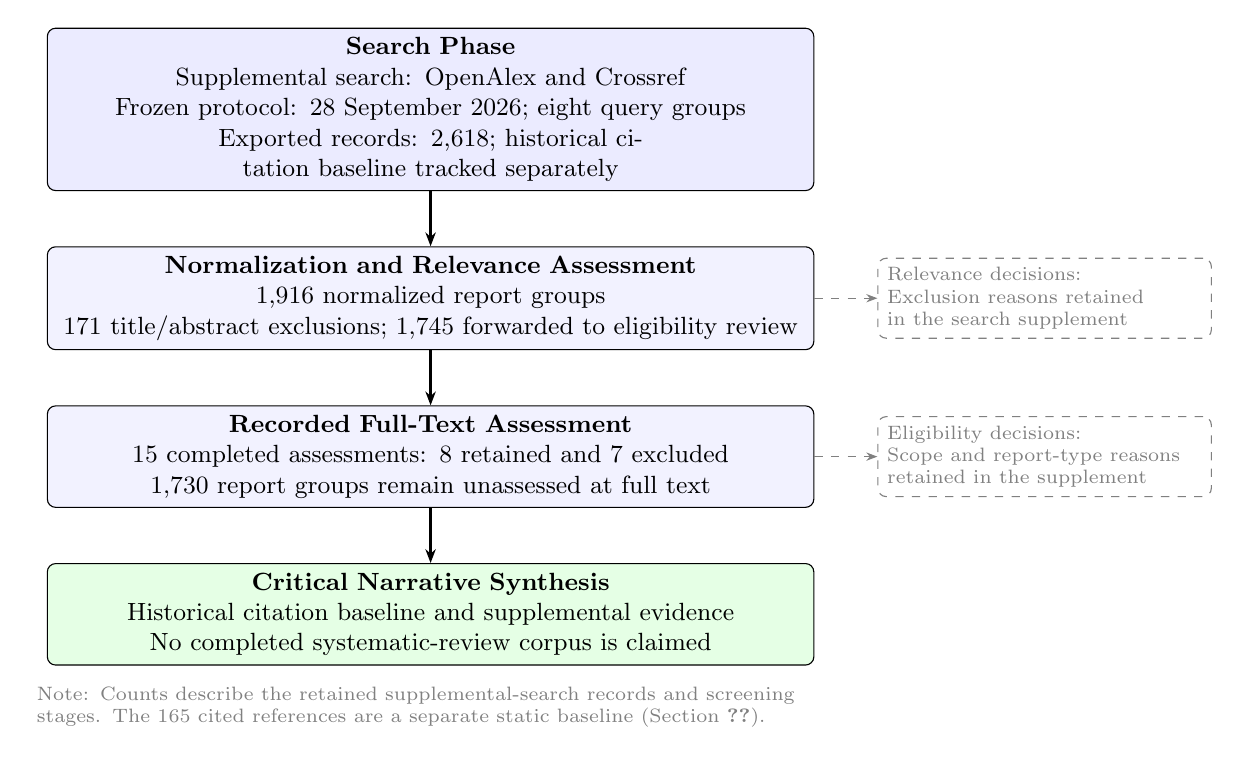
\begin{tikzpicture}[
  node distance=0.7cm,
  box/.style={rectangle, draw=black, rounded corners=3pt,
              text width=9.5cm, align=center,
              minimum height=0.9cm, font=\small},
  excl/.style={rectangle, draw=gray, dashed, rounded corners=3pt,
               text width=4.0cm, align=left,
               minimum height=0.9cm, font=\scriptsize, text=gray},
  arr/.style={-{Stealth[length=5pt]}, thick},
  exclarr/.style={-{Stealth[length=4pt]}, gray, dashed}
]
\node[box, fill=blue!8] (id)
  {\textbf{Search Phase}\\
   Supplemental search: OpenAlex and Crossref\\
   Frozen protocol: 28 September 2026; eight query groups\\
   Exported records: 2,618; historical citation baseline tracked separately};

\node[box, fill=blue!5, below=of id] (screen)
  {\textbf{Normalization and Relevance Assessment}\\
   1,916 normalized report groups\\
   171 title/abstract exclusions; 1,745 forwarded to eligibility review};
\node[box, fill=blue!5, below=of screen] (fulltext)
  {\textbf{Recorded Full-Text Assessment}\\
   15 completed assessments: 8 retained and 7 excluded\\
   1,730 report groups remain unassessed at full text};
\node[box, fill=green!10, below=of fulltext] (final)
  {\textbf{Critical Narrative Synthesis}\\
   Historical citation baseline and supplemental evidence\\
   No completed systematic-review corpus is claimed};
\node[excl, right=0.8cm of screen] (excl1)
  {Relevance decisions:\\
   Exclusion reasons retained\\
   in the search supplement};
\node[excl, right=0.8cm of fulltext] (excl2)
  {Eligibility decisions:\\
   Scope and report-type reasons\\
   retained in the supplement};

\draw[arr] (id) -- (screen);
\draw[arr] (screen) -- (fulltext);
\draw[arr] (fulltext) -- (final);
\draw[exclarr] (screen.east) -- (excl1.west);
\draw[exclarr] (fulltext.east) -- (excl2.west);

\node[font=\scriptsize, text=gray, below=0.15cm of final, text width=10cm, align=left]
  {Note: Counts describe the retained supplemental-search records and screening stages.
   The 165 cited references are a separate static baseline (Section~\ref{sec:method}).};
\end{tikzpicture}
\caption{Recorded supplemental-search stages accompanying the narrative survey. Counts are report-level; the supplemental search is capped and full-text coverage is incomplete.}
\label{fig:prisma}
\end{figure}

To further constrain quantitative claims, Table~\ref{tab:evidence_matrix} lists
the evidence sources and applicable conditions for the paper's core numerical
findings. Beyond data explicitly reported in the original papers, we do not
extrapolate values from public talks, drafts, or secondary sources into general
conclusions. Heterogeneity across studies---arising from differences in testbed
type, statistical metrics, AQM configuration, and BBRv1 kernel version---is
particularly notable for AQM configuration: \citet{pokhrel2025wifi} showed that
FQ-CoDel can raise the inter-flow Jain fairness index between BBRv3 and CUBIC
from approximately 0.6 to approximately 0.9. We annotate AQM configuration
information in relevant scenario analyses; for papers that do not report
configuration, caveats on the generalizability of their conclusions apply.

\begin{table}[pos=tbp]
  \caption{Source and condition mapping for scenario comparisons.}
  \label{tab:evidence_matrix}
  \small
  \begin{tabularx}{\tblwidth}{@{}p{4.2cm}p{2.8cm}X@{}}
    \toprule
    \textbf{Reported comparison} & \textbf{Source} & \textbf{Applicable conditions} \\
    \midrule
    Backbone throughput improvements reported under source-specific path and host conditions &
      \citet{cardwell2017bbr} &
      Google production WAN with open receive buffers; not generalized to all public paths \\
    BBR shows throughput degradation or queuing anomalies under shallow-buffer/high-loss conditions &
      \citet{cao2019bbr,jaeger2019bbr} &
      Valid within controlled testbed parameter ranges; requires interpretation with buffer and loss source \\
    BBRv3/CUBIC throughput depends on the evaluated configuration &
      \citet{gomez2024bbrv3} &
      Real broadband testbed with reported AQM/path configuration; not representative of all broadband ISPs \\
    BBRv3/CUBIC coexistence can exhibit strongly unequal shares &
      \citet{abrol2026bbr,zeynali2024bbrv3} &
      Extreme fairness cases in large-buffer or specific real paths; used to illustrate risk boundaries \\
    Standard BBR may underperform CUBIC in WiFi frame-aggregation; BBRp partially mitigates loss &
      \citet{grazia2020bbrp} &
      802.11n/ac test conditions; not directly extrapolated to all WiFi~6/7 deployments \\
    BBR outperforms CUBIC on Starlink-class LEO links; QUIC+BBR handover optimization &
      \citet{deutschmann2023starlink,kamel2024starquic} &
      Specific satellite, geography, terminal, and handover mode; independent replication still needed \\
    \bottomrule
  \end{tabularx}
\end{table}

\subsection{Contributions and Paper Organization}
\label{sec:contrib}

The survey addresses three connected questions: which path and
implementation conditions are needed to interpret BBR results; which
mechanism claims can explain measured allocation without mistaking a
rate--delay identity for a share law; and how evidence can support a
metric-specific performance assessment.

Our first contribution is a conditional organization of BBRv1--v3 evidence
across six scenario groups. It separates direct BBR evaluations, mechanism
materials and supporting transport context, and supplies a reference-level
traceability register and the retained supplemental-search records.
This differs from a coverage-only comparison by keeping the conditions
needed to interpret throughput, delay, fairness and retransmissions.
Bringing these scenarios into a common assessment reveals which inputs
and metrics are needed to interpret results across configurations.

Our second contribution is an analytical assessment procedure
(Section~\ref{sec:analytical_assessment}). It demonstrates the
non-identifiability of bandwidth shares from the in-flight identity,
expresses two-flow fairness requirements as share constraints, and gives
explicit requirement-dependent outputs including undetermined cases.
The underlying BDP and Jain identities are established; the contribution
is their use in a reproducible assessment with stated inputs, windows and
service requirements.

Our third contribution is a 340-run controlled comparison with
implementation identities, measurement definitions and reproducible data.
Besides RTT asymmetry, BBR/CUBIC coexistence, additional equal-RTT cases
and artificial loss, we quantify a retrospective transfer test from E1
calibration to disjoint E3 runs. Prediction errors against a constant baseline quantify the dependence
of transfer estimates on queue conditioning. The learning-control discussion separates objectives,
measured outcomes and deployment evidence.

Section~\ref{sec:algo} presents the controller foundations and version
differences. Section~\ref{sec:framework} defines the framework and analytical
assessment. Sections~\ref{sec:comparison} and \ref{sec:fairness} synthesize
scenario and fairness evidence; Section~\ref{sec:deployment} examines
learning-assisted control. Section~\ref{sec:controlled_experiments} gives the
experiments and transfer evaluation, and Section~\ref{sec:conclusion}
states the resulting conclusions and limits.

% ============================================================
\section{BBR Algorithm Foundations and Version Evolution}
\label{sec:algo}
% ============================================================

\subsection{Measurement Model and Sending Control}
\label{sec:design}

Understanding BBR's applicability boundaries requires first understanding the
network model on which its design rests---BBR's advantages and limitations both
stem from the same set of measurement assumptions.

BBR models the path using estimates of bottleneck bandwidth (BtlBw) and
propagation delay (RTprop). Their product provides a reference in-flight
volume for the ``just filling the pipe'' operating target
\citep{cardwell2017bbr,kleinrock1979power}. In the BBRv1 design, delivery-rate
samples feed a maximum filter over ten packet-timed rounds, and RTT samples
feed a minimum filter with a ten-second window. These estimates can be
affected by application or receiver limits, ACK timing, queueing and path
changes. Filter horizons and update rules must be checked
against the particular version and implementation rather than transferred
unchanged to BBRv2 or BBRv3~\citep{cardwell2017bbr,cardwell2019bbrv2,paxson1999dynamics}.
Figure~\ref{fig:optimal_point} illustrates this operating target and the
underutilization/bufferbloat trade-off around the BDP point.

\begin{figure}[pos=htbp]
  \centering
  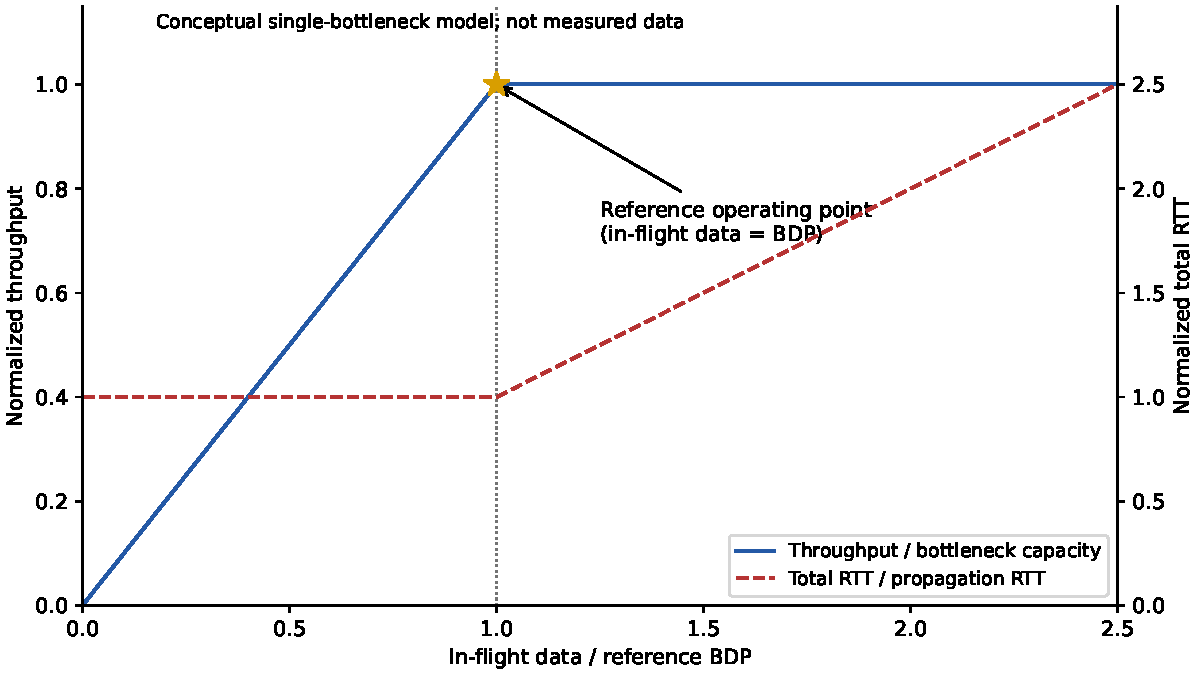
\includegraphics[width=0.62\columnwidth]{optimal_operating_point_corrected.pdf}
  \caption{Conceptual operating point for a single bottleneck. Throughput saturates when in-flight data reaches the reference BDP. Propagation RTT is held constant; additional queue occupancy increases total RTT through queueing delay. Curves are illustrative, not measured data.}
  \label{fig:optimal_point}
\end{figure}

A classical approximation for a Reno-like additive-increase,
multiplicative-decrease flow is
\begin{equation}
  \label{eq:mathis}
  \mathrm{BW}_{\mathrm{Reno}} \approx
  \frac{K \cdot \mathrm{MSS}}{\mathrm{RTT}\cdot\sqrt{p}}.
\end{equation}
Here $p$ denotes loss probability and $K$ depends on modeling assumptions,
including acknowledgment behavior~\citep{mathis1997macroscopic}. The
approximation describes a restricted steady-state regime and does not
account for all timeout, receiver-window or application limitations.
CUBIC has a different window evolution~\citep{ha2008cubic}. The Reno-like
approximation motivates examining RTT and loss jointly within its stated
steady-state regime.

A simplified BBRv1 model relates pacing and the target congestion window
to these estimates:
\begin{gather*}
  \mathrm{pacing\_rate}_{\mathrm{target}} =
  \mathrm{BtlBw} \times \mathrm{pacing\_gain} \\[2pt]
  \mathrm{cwnd}_{\mathrm{target}} \approx
  \mathrm{BtlBw} \times \mathrm{RTprop} \times \mathrm{cwnd\_gain}.
\end{gather*}
These are controller targets, not exact identities for the instantaneous
Linux congestion window. Recovery, minimum-window rules, packetization,
ACK aggregation and host limits can change the realized behavior.
Pacing spreads transmissions in time~\citep{aggarwal2000pacing}, while the
congestion window limits outstanding data~\citep{semke1998buffer}; queue overflow depends on their interaction with the available buffer.

The BBRv1 design has four principal modes (Figure~\ref{fig:bbr_arch}).
Startup seeks additional delivery rate; its full-bandwidth test checks
whether estimated bandwidth has grown by at least 25\% over three
consecutive packet-timed rounds. Drain reduces the excess in-flight data
accumulated during Startup. ProbeBW varies pacing gain to probe and drain,
and ProbeRTT temporarily reduces the congestion window to obtain a less
queue-inflated RTT sample~\citep{cardwell2017bbr}. These modes do not all
recur periodically, and ProbeRTT does not guarantee a queue-free sample.
Later versions revise the probing and in-flight constraints. ECN response
must likewise be identified from the specific implementation and actual
configuration; support for an ECN mechanism does not prove that it was
enabled in a reported experiment~\citep{rfc3168,cardwell2019bbrv2}.

\begin{figure}[pos=htbp]
  \centering
  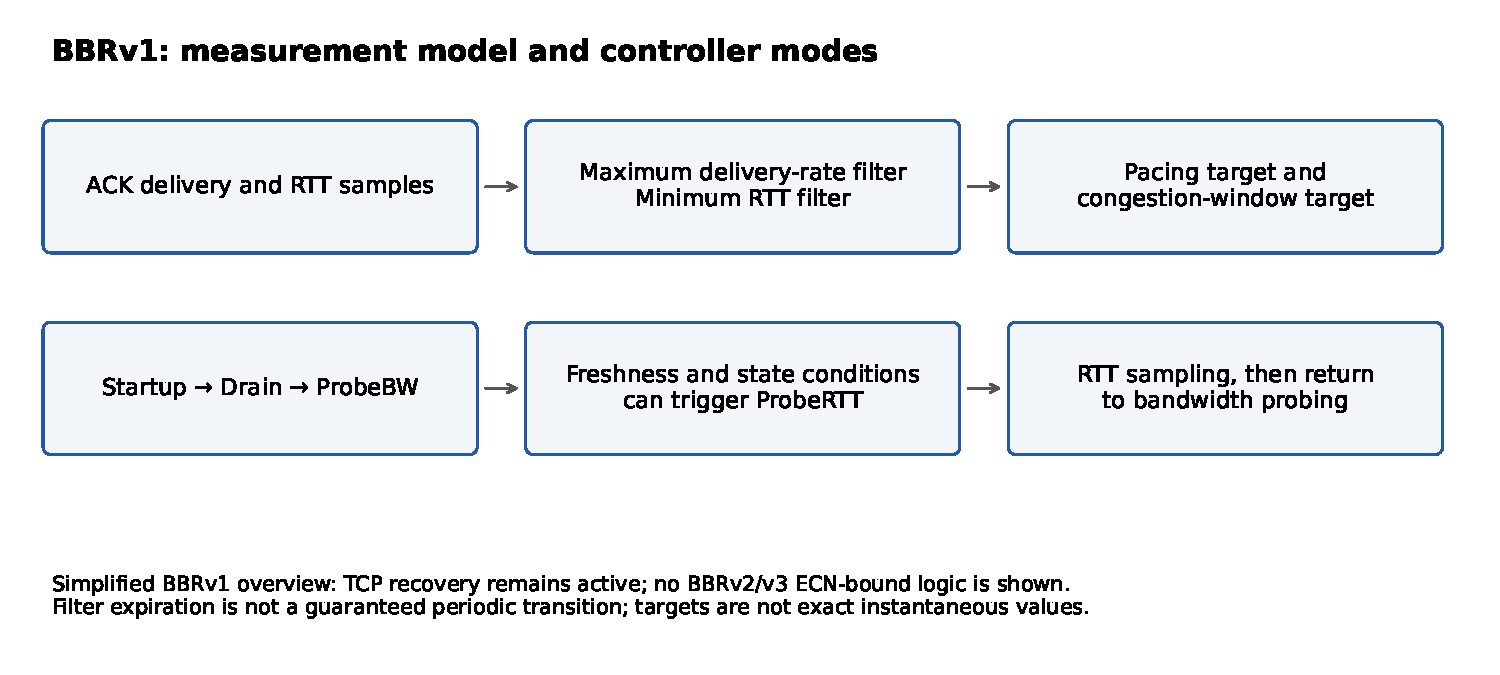
\includegraphics[width=\columnwidth]{bbr_architecture_corrected.pdf}% filename confirmed
  \caption{Simplified BBRv1 measurement and control architecture. Delivery-rate and RTT samples inform pacing and congestion-window targets. ProbeRTT entry depends on freshness and state conditions, rather than a fixed periodic timeout. Later-version ECN-bound mechanisms are not part of this BBRv1 diagram. The original figure was generated with GPT Image 2.0 and manually checked by the authors; this replacement was drawn with Python/matplotlib using AI-assisted code preparation.}
  \label{fig:bbr_arch}
\end{figure}

\subsection{Core Differences Across Three Versions}
\label{sec:evolution}

BBR's evolution from BBRv1 in 2016~\citep{cardwell2017bbr}, through BBRv2 in
2019~\citep{cardwell2019bbrv2}, to the BBRv3 draft in
2023~\citep{cardwell2023bbrv3}, retains a delivery-rate and propagation-delay model while revising
congestion responses and probing. The comparison below covers three
mechanism groups: tightening Startup exit conditions, restructuring
ProbeBW, and tuning ProbeRTT parameters. Figure~\ref{fig:version_compare}
provides the visual summary, while Table~\ref{tab:versions} compares the key
parameters.

\paragraph{Startup Exit Conditions}
BBRv1's full-bandwidth test uses insufficient estimated bandwidth growth
across non-application-limited packet-timed rounds. Later versions add
congestion-related exit conditions~\citep{cardwell2019bbrv2,cardwell2023bbrv3}.
In the inspected BBRv3 source, the loss-based check requires a Recovery
round boundary, at least six loss-marking events in that round and an
excessive in-flight loss indication. Six events are not simply six lost
packets. The ECN-based check requires an eligible connection and two
consecutive rounds meeting the configured CE-ratio threshold. These checks
cannot be reduced to an unconditional packet-count trigger or a claim of
improved fairness without measurements.

\paragraph{ProbeBW Structure}
BBRv1 uses an eight-phase gain sequence (1.25, 0.75, 1.0$\times$6).
Phase duration depends on elapsed minimum-RTT time, in-flight data and loss
conditions; it is not exactly eight packet-timed rounds. BBRv2/v3 restructure this into four sub-phases---Refill/Up/Down/Cruise---introducing
two dynamic bounds $\mathrm{inflight\_hi}$ and
$\mathrm{inflight\_lo}$~\citep{cardwell2019bbrv2}. The inspected BBRv3 source sets the Down gain with the integer expression
$\lfloor256\times91/100\rfloor/256=232/256$. This gives the source-specific drain gain~\citep{cardwell2023bbrv3};
coexistence is evaluated through measured per-flow rates.

\paragraph{ProbeRTT}
ProbeRTT entry depends on the implementation's RTT-sample freshness and
state conditions; a filter window is not an unconditional periodic timer.
The inspected BBRv3 source distinguishes a ten-second minimum-RTT filter
from a five-second ProbeRTT sampling window, with a half-BDP target
subject to the minimum congestion window. These parameters do not by
themselves establish how much bandwidth a competing CUBIC flow obtains.
The exact source revision and runtime conditions must accompany a
version-specific comparison~\citep{cardwell2019bbrv2,cardwell2023bbrv3}.

QUIC implementations can also use BBR. QUIC runs over UDP and lets
applications implement congestion control without changing the kernel TCP
controller~\citep{rfc9000}. BBR's behavior specification in QUIC is
now maintained by the IETF CCWG working group
draft~\citep{ietf_ccwg_bbr}. However, the QUIC+BBR combination also introduces
new fairness issues, as multiple QUIC connections are treated by the OS as
independent UDP flows whose aggregate behavior differs from native TCP
flows~\citep{abrol2026bbr}.

\begin{figure}[pos=htbp]
  \centering
  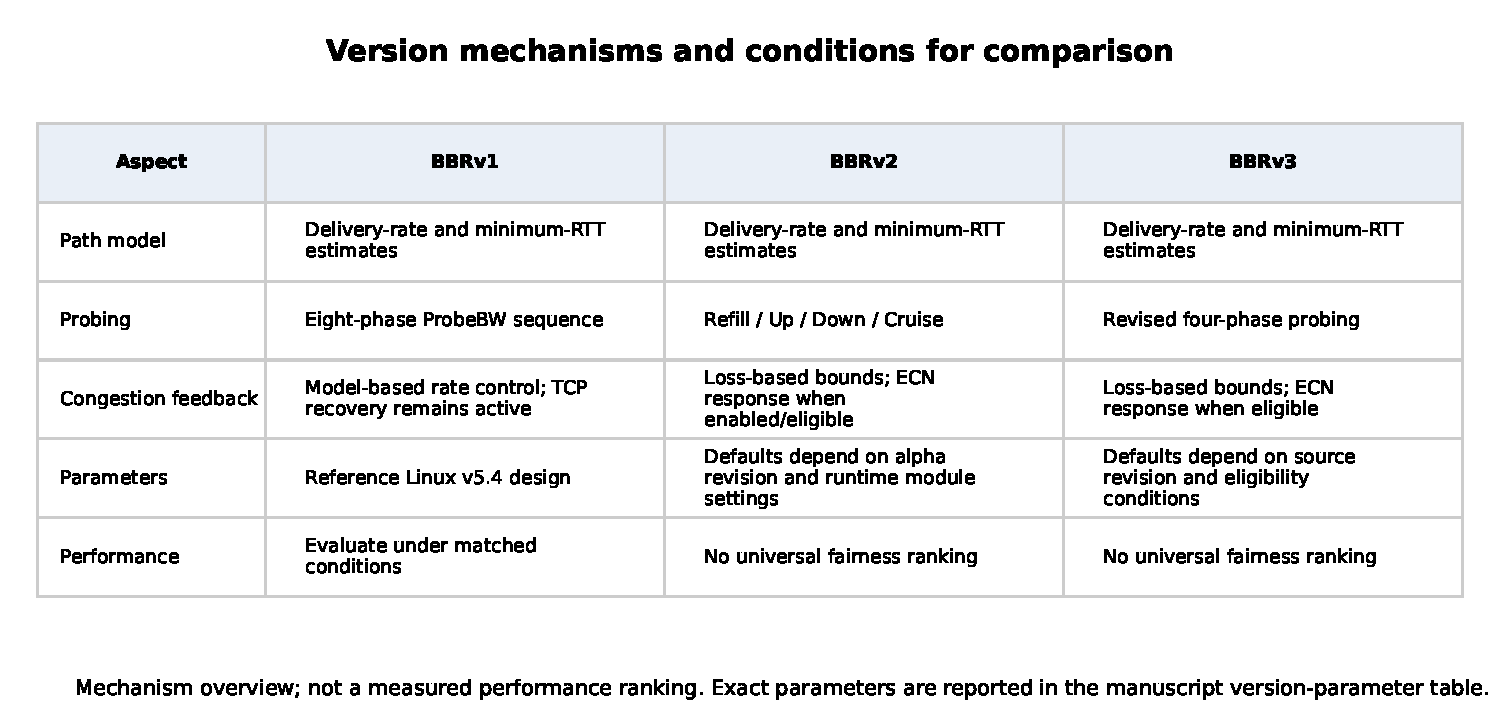
\includegraphics[width=\columnwidth]{version_comparison_corrected.pdf}% filename confirmed
  \caption{Version-specific mechanisms and comparison conditions. The overview does not imply monotonic improvement in throughput, delay or fairness; source-specific parameters are reported in Table~\ref{tab:versions}. The original figure was generated with GPT Image 2.0 and manually checked by the authors; this replacement was drawn with Python/matplotlib using AI-assisted code preparation.}
  \label{fig:version_compare}
\end{figure}

\begin{table}[pos=tbp]
  \caption{Key parameter comparison of BBRv1/v2/v3
    \citep{cardwell2017bbr,cardwell2019bbrv2,cardwell2023bbrv3,abrol2026bbr}.}
  \label{tab:versions}
  \small
  \begin{threeparttable}
  \begin{tabularx}{\tblwidth}{@{}p{2.8cm}XXX@{}}
    \toprule
    \textbf{Parameter} & \textbf{BBRv1} & \textbf{BBRv2} & \textbf{BBRv3} \\
    \midrule
    Startup exit &
      BW gain ${<}25\%$ (3 rounds) &
      BW-growth test plus conditional loss/ECN exits; 8 loss events in inspected alpha source &
      BW-growth test plus conditional loss/ECN exits; 6 loss events in inspected source \\
    \midrule
    ProbeBW structure &
      8-phase sequence (1.25, 0.75, 1.0$\times$6) &
      Refill/Up/Down/Cruise sub-phases &
      Four sub-phases; Down gain is revision-dependent \\
    \midrule
    ProbeRTT target     & 4\,MSS    & $\max(4\,\mathrm{MSS},\mathrm{BDP}/2)$ & $\max(4\,\mathrm{MSS},\mathrm{BDP}/2)$ \\
    ProbeRTT freshness window & 10\,s (v1 design) & 5\,s (inspected alpha source) & 5\,s (inspected source)  \\
    $\mathrm{cwnd\_gain}$ & 2.0 (baseline) & State-dependent & State-dependent \\
    $\mathrm{pacing\_gain}$ (Down) & 0.75 & 0.75 & $232/256$ (inspected source) \\
    ECN support & None & Implemented; disabled by default in inspected alpha source & Conditional on ECN eligibility \\
    $\mathrm{inflight\_hi}$ constraint & None & Yes & Yes \\
    Primary goal & Baseline & Fairness \& ECN & Reduce queue; relieve starvation \\
    \bottomrule
  \end{tabularx}
  \begin{tablenotes}
    \small
    \item For BBRv2/v3, ECN marking provides an additional network-side signal (RFC~3168~\citep{rfc3168}).
    In both inspected source snapshots, the loss counter counts marking events, not lost packets.
    These source defaults are distinguished from the identities of the experimental builds.
    ECN sender eligibility additionally checks negotiated capability and an RTT condition.
    Filter and freshness windows are not unconditional ProbeRTT entry intervals.
    When ECN marking is unavailable, ECN-derived feedback is absent, but loss-driven
    bound updates and the associated state-control logic remain active. The absence
    of ECN alone therefore does not imply reversion to BBRv1; parameter values and
    behavior remain implementation- and state-dependent.
  \end{tablenotes}
  \end{threeparttable}
\end{table}

\FloatBarrier

% ============================================================
\section{Three-Dimensional Applicability Framework}
\label{sec:framework}
% ============================================================

BBR measurements differ across path conditions and implementations. This
section organizes those conditions using buffer depth, BDP magnitude and
loss source, with implementation, queue management and competing flows
reported alongside them. The framework connects these inputs to separate
throughput, delay, fairness and retransmission requirements. Measured flow
rates provide the allocation evidence, while the analytical assessment and
quantitative transfer comparison show how the inputs are interpreted.

\subsection{Framework Design Motivation}

BBR's strong dependence on network conditions indicates that a single-dimensional
performance metric cannot effectively predict its behavior in unknown environments.
Measurements by \citet{medina2004transport} show that transport protocol behavior
varies greatly with network environment evolution; \citet{barakat2000tcp} further
reveals that TCP behavior is highly dependent on path characteristics in
heterogeneous networks. We therefore propose a BBR applicability boundary
analysis framework composed of three related physical dimensions, mapping BBR's
behavioral characteristics under different network conditions to a unified
coordinate space.

\subsection{Three-Dimensional Definitions and Physical Meaning}
\label{sec:framework_dim}

The three dimensions reflect BBR's path model and the network conditions
that affect its estimates and control responses. Their working numerical
bins organize the evidence; they are not derived physical laws.

\textbf{Buffer depth} (measured in BDP units; this paper uses working bins of
shallow $<1.5\times$BDP, medium $1.5$--$10\times$BDP, and deep $>10\times$BDP)
is an analysis dimension rather than a universal physical boundary. The theoretical
basis comes from Kleinrock's optimal power theory~\citep{kleinrock1979power}: BBR
targets ``just-full pipe'' sending, periodically reducing cwnd during ProbeRTT to
obtain queue-free RTprop estimates, and the relative cost of this active
yielding depends on queue depth, RTT, competing traffic and implementation.
Shallow buffers can expose probing-induced loss, while larger buffers can
increase queueing delay. Neither buffer depth nor ProbeRTT alone fixes the
resulting bandwidth shares~\citep{appenzeller2004sizing,dhamdhere2006buffer,wischik2005buffers}.
Queue management and per-flow scheduling, including FQ-CoDel,
change these interactions~\citep{hoeiland2018fq}.

\textbf{BDP magnitude} (measured by the $\mathrm{BW}\times\mathrm{RTT}$ product;
the working bins in this review use low $<1$\,MB and high $>10$\,MB) organizes
capacity and delay conditions. Paths with the same BDP may have different
RTTs, capacities, loss processes and controller behavior. The Reno-like
approximation in Eq.~(\ref{eq:mathis}) therefore does not establish a BDP-only
throughput ceiling or a guaranteed advantage for BBR.

\textbf{Loss source} (congestion-induced / random / mixed) matters because
packet loss alone does not identify its cause. BBRv1 primarily regulates
sending through its delivery-rate and propagation-delay model, while
BBRv2 and BBRv3 also use loss-related constraints. TCP recovery remains
necessary in all versions. Random loss can reduce delivered goodput and
increase retransmission overhead; its effect depends on implementation,
queueing, link-layer recovery and workload. The WiFi experiments of
\citet{grazia2020bbrp} further show why sender location, chipset and host
queue settings must accompany a wireless comparison. Loss assessment combines controller responses with link-layer recovery,
queue policy and workload.

\paragraph{Theoretical Basis for Thresholds}
The threshold values are working bins anchored to prior measurements and
theoretical reasoning, rather than universal cutoffs. The buffer-depth bins
summarize patterns reported by \citet{cao2019bbr} and \citet{jaeger2019bbr};
their effects depend on version, queue management, RTT, and flow count. BDP
magnitude thresholds of 1\,MB (low) and 10\,MB (high) are also working bins,
not universal boundaries. They organize the discussion and are not derived
as performance transition points from Eq.~(\ref{eq:mathis}). A numerical
transition requires evidence for the specified version, workload and path.

\subsection{Six-Scenario Positioning}
\label{sec:framework_pos}

Table~\ref{tab:framework} maps the six representative scenarios covered in this
paper to the three-dimensional coordinate system.

\begin{table}[pos=tbp]
  \caption{Positioning of six network scenarios in the three-dimensional
    applicability boundary framework.}
  \label{tab:framework}
  \small
  \begin{tabularx}{\tblwidth}{@{}p{2.1cm}p{1.3cm}p{1.2cm}p{1.5cm}p{1.6cm}X@{}}
    \toprule
    \textbf{Scenario} & \makecell[l]{\textbf{Buffer}\\\textbf{depth}} & \textbf{BDP}
      & \makecell[l]{\textbf{Loss}\\\textbf{source}} & \makecell[l]{\textbf{Scope}}
      & \textbf{Key constraint} \\
    \midrule
    High-BDP WAN & Medium & High & Congestion & Throughput & Recv.\ buffer $\geq$ BDP \\
    Shallow-buf.\ wired & Shallow & Low & Congestion & Loss cost & Retransmission surge \\
    Broadband multi-flow & Medium & Medium & Congestion & Coexistence & Fairness varies with queue \\
    High-loss wireless & Medium & Low--Med & Random & Link/host & WiFi frame aggregation \\
    High-dynamic routing & Medium & Medium & Mixed & Adaptation & Multi-path fairness unverified \\
    LEO satellite & Variable & Varies & Mixed & Dynamics & RTT spikes, BW asymmetry \\
    \bottomrule
  \end{tabularx}
\end{table}

\subsection{Decision Rules and Known Limitations}
\label{sec:framework_rules}

The framework provides a condition-specific assessment procedure with
explicit inputs and separate performance outputs. Its inputs are bottleneck
capacity, the reference RTT used for BDP, absolute buffer size, loss source,
BBR version, queue management and flow count. For heterogeneous flows, the reference RTT and each
flow's RTT are reported separately. Its outputs are four separate assessments:
throughput, delay, bandwidth fairness, and retransmission cost. A missing input
or insufficient evidence produces ``undetermined'' rather than a forced rating.
The working buffer bins are shallow $<1.5\times$BDP, medium
$1.5$--$10\times$BDP, and deep $>10\times$BDP; these bins organize the reviewed
evidence and are not universal physical thresholds.

Based on these conditional rules, Table~\ref{tab:decision_rules} summarizes
scenario-level expectations and known counter-examples. The entries are evidence
summaries, not guarantees for an arbitrary deployment.

\begin{table}[pos=tbp]
  \caption{Three-dimensional framework decision rules and known counter-examples.}
  \label{tab:decision_rules}
  \small
  \begin{tabularx}{\tblwidth}{@{}p{3.8cm}p{1.0cm}p{1.3cm}p{1.6cm}X@{}}
    \toprule
    \textbf{Typical condition} & \textbf{Buf.} & \textbf{BDP} & \makecell[l]{\textbf{Loss}\\\textbf{source}}
      & \textbf{Conditional expectation} \\
    \midrule
    High-BDP backbone (recv.\ buf.\ $\geq$BDP) & Med & $>$10\,MB & Cong.
      & Throughput advantage is plausible when receive buffer $\geq$BDP; delay, fairness, and retransmission require separate checks \\
    \midrule
    Wired multi-flow (1.5--$10\times$BDP buf.) & Med & Med & Cong.
      & Throughput may improve; fairness remains conditional on RTT, queue, version, and flow count \\
    \midrule
    Deep-buffer wired ($>10\times$BDP) & Deep & Any & Cong.
      & Deep buffers can change the BBR/CUBIC share and increase queueing delay; exact fairness is configuration-dependent \\
    \midrule
    WiFi 802.11n/ac (standard BBR) & Med & Low--Med & Random
      & Pacing, TSQ, chipset, direction and queue policy affect frame aggregation; a scalar BBR/CUBIC ratio is not transferable \\
    \midrule
    LEO satellite (Starlink-class) & Varies & Varies & Mixed
      & High-BDP benefit may be offset by RTT variation, random loss, and path dynamics; evidence is insufficient for a fixed rating \\
    \midrule
    Shallow-buf.\ wired ($<1.5\times$BDP) & Shal & Low & Cong.
      & Bandwidth share and retransmissions require source-specific queue/RTT conditions \\
    \bottomrule
  \end{tabularx}
  \begin{tablenotes}
    \small
    \item The WiFi row marks a known framework boundary:
    802.11 frame aggregation is a protocol-layer constraint that cannot be mapped to the
    three physical dimensions; variants such as BBRp can partially remedy this through
    controlled bursts.
  \end{tablenotes}
\end{table}

\subsection{Analytical Assessment and Identifiability}
\label{sec:analytical_assessment}

The framework distinguishes a description of the path from a decision about
performance. We formalize this distinction using a condition vector
$z=(C,R_*,\{R_i\},Q,L,v,A,n,W)$: bottleneck capacity, reference and
per-flow propagation RTTs, absolute queue limit, loss process, implementation,
queue policy, flow count and observation window. The physical descriptors are
$\mathrm{BDP}_*=CR_*$ and $q=Q/(CR_*)$, with capacity and queue expressed
in consistent bit units. These descriptors organize cases; the following
analysis shows why they cannot determine bandwidth allocation by themselves.

\paragraph{Allocation is not identified by the in-flight identity.}
For two flows, let their aggregate rate be $0<G\leq C$ and let $s$ be the
second flow's share. The rates $x_1=(1-s)G$ and $x_2=sG$ satisfy the same
aggregate-rate constraint for every $s\in[0,1]$. Their propagation-pipe
amounts $I_i=x_iR_i$ also satisfy the per-flow rate--delay identities.
Thus, even with $C,R_1,R_2,Q$ fixed, the identities admit different shares;
a longer propagation RTT does not algebraically force a larger share.
This is an identifiability result about the equations, not a claim that all
shares are equilibria of a particular controller. Selecting the realized
allocation requires controller and queue dynamics or direct measurements.

\paragraph{Utilization and fairness are separate constraints.}
Define normalized receiver goodput $u=G/C$ and imbalance
$d=|2s-1|$. Substituting the two rates into Jain's standard index
\citep{jain1984fairness} gives
\begin{equation}
 J=\frac{1}{2\{s^2+(1-s)^2\}}=\frac{1}{1+d^2}.
 \label{eq:share_jain}
\end{equation}
Consequently, a fairness requirement $J\geq j_0$, where
$1/2\leq j_0\leq1$, is equivalent to
\begin{equation}
 \frac{1-\sqrt{j_0^{-1}-1}}{2}\leq s\leq
 \frac{1+\sqrt{j_0^{-1}-1}}{2}.
 \label{eq:share_acceptance}
\end{equation}
For example, $j_0=0.95$ requires a share between 0.385 and 0.615,
regardless of whether aggregate goodput fills the link. Jain's index and
this algebraic transformation are established metrics, not new fairness
measures. Our analytical contribution is to use their explicit feasible
region to separate path descriptors, performance requirements and observable
allocation in a BBR assessment.

\paragraph{A requirement-dependent assessment procedure.}
A workload specifies its requirements before protocol selection: a minimum
$u_0$, a minimum $j_0$, a delay limit $D_0$, and a retransmission budget
$H_0$. For each required metric, the assessment returns \emph{meets},
\emph{does not meet}, or \emph{undetermined}. A missing or incompatible
measurement window yields \emph{undetermined}, rather than an inferred pass.
A joint assessment meets the requirements only if every required metric
meets its own limit. An observed violation yields a failure for that
requirement; if there is no observed violation but some required evidence is
missing, the joint result remains undetermined. A zero-goodput run has $u=0$ and undefined Jain fairness; it cannot pass
a positive utilization requirement. This procedure allows
throughput and fairness evidence to be usable without claiming that they
establish latency or retransmission suitability.

For repeated runs, we report both metric means and the empirical fraction
satisfying the joint rate/share conditions:
\begin{equation}
 \widehat p_{u,J}=\frac{1}{N}\sum_{r=1}^{N}
 \mathbf{1}\{u_r\geq u_0,\ J_r\geq j_0\}.
 \label{eq:assessment_fraction}
\end{equation}
The fraction is descriptive with five repetitions per condition; it is not
a population reliability guarantee. Equation~\ref{eq:share_jain} is applied
within each run. In general, substituting an averaged share does not recover
the mean Jain index. Queue bins and BDP bins do not set $u_0,j_0,D_0,H_0$:
those limits express service requirements and must be reported separately.
Section~\ref{sec:framework_transfer} evaluates the rate/fairness component
and its transfer limitations using the archived measurements.


\subsection{External Consistency Check of the Framework}
\label{sec:framework_valid}

To assess external consistency, we compare the conditional expectations
with published measurements outside our controlled experiment matrix.
The Scholz measurements provide an external comparison for the relationships
among capacity, RTT, queue depth and allocation. They were part of the
evidence used to organize the framework, so the comparison is interpreted
through its reported conditions.

The comparison asks whether reported behavior is compatible with three
conditional expectations: throughput differences can depend on BDP and
receive-buffer constraints; deep queues can affect BBR/CUBIC allocation;
and changing capacity and RTT can alter the comparison. We do not require
a fixed throughput multiple, a universal share threshold, or a monotonic
performance ratio as BDP increases.

\citet{scholz2018deeper} examine BBR and CUBIC under varied bottleneck
bandwidths, RTTs and buffer settings in a controlled testbed. Their
configuration-dependent observations motivate reporting these inputs
together. This provides an external consistency comparison, not a held-out
test of predictive accuracy: the study also informed the framework's
organization. The controlled experiments in Section~\ref{sec:controlled_experiments}
provide additional measurements with explicit inputs and metric definitions.

The dimensions are related: high BDP and deep buffering can co-occur,
and the observed loss process changes with load and queue management.
Flow count and RTT heterogeneity also affect sharing. We therefore record
implementation, AQM and competing flows alongside the three dimensions
and assess throughput, delay, fairness and retransmissions separately.

% ============================================================
\section{Multi-Scenario Performance Evaluation}
\label{sec:comparison}
% ============================================================

BBR performance depends on both network conditions and implementation.
Wired backbone measurements and WLAN experiments use different link,
queue, pacing and host configurations, so their throughput ratios are
not interchangeable. This section examines six scenario groups while
retaining those source-specific conditions. Source-specific
measurements are reported in the corresponding scenario subsections and
Table~\ref{tab:summary}; high-dynamic routing is treated
qualitatively because comparable version-by-version throughput ratios are not
available.

\subsection{Scenario 1: High-BDP Wide-Area Networks}
\label{sec:wan}

High-BDP WANs can expose differences between path-model-based and
loss-driven congestion control. Their performance depends on RTT, loss,
receiver-window limits and implementation, rather than BDP alone.
\citet{cardwell2017bbr} report improvements for BBR in their backbone
measurements. Those measurements connect the reported throughput improvements to their
path and host conditions.

Sustaining a target rate also requires a receive window large enough for
the corresponding rate--RTT product.
The original paper's controlled experiment shows that once the receive window is
limited, BBR's algorithmic advantage is masked by the receiver bottleneck and
throughput drops to levels comparable to CUBIC~\citep{cardwell2017bbr}.

\subsection{Scenario 2: Shallow-Buffer Wired Networks}
\label{sec:shallow}

Shallow-buffer comparisons must report absolute queue size, capacity,
reference RTT, implementation and flow count together. A queue size in
kilobytes cannot be compared across studies without those conditions.
The cited Cao and Jaeger studies use different configurations, so their
observations are not combined into a single queue-sweep table here
\citep{cao2019bbr,jaeger2019bbr}.

The inspected Jaeger author manuscript reports a configuration-dependent
relationship between buffer size and BBR/CUBIC shares. Its Figure~10 uses
both common-RTT and asymmetric-RTT experiments; those observations do
not establish a universal retransmission multiplier or a fixed suitability
rating. When interpreting competition, distinguish the TCP recovery logic
from the congestion controller's response to loss, and report receiver
goodput separately from retransmission counts. Applications with different
latency, delivery and retransmission requirements may assess the same
configuration differently.

\citet{cao2019bbr} report a sharp goodput decline near 20\% configured
random loss in their 100-Mbps, 25-ms, 10-MB-buffer experiment. This
source-specific loss sweep does not establish that BBR is generally
unaffected below 20\% loss, or transfer that boundary to later versions.

\FloatBarrier

\subsection{Scenario 3: Stable Broadband Multi-Flow (BBRv3 Benchmark)}
\label{sec:bbr3}

\citet{gomez2024bbrv3} evaluate BBRv3 using distinct emulated and
hardware configurations. The reported comparisons vary with loss, RTT,
buffer size, competing flows and queue management; they should not be
summarized as a fixed throughput multiplier over CUBIC.

In the emulated loss sweep (Section~5.4, Figure~7), the study uses a
1-Gbps bottleneck, a reported 20-ms propagation delay, a BDP-sized buffer,
and ten 120-s runs per loss rate. BBRv2 and BBRv3 throughput declines
noticeably above 0.1\% loss and reaches about 60\% of its maximum at
0.5\% loss. The reported throughput remains above 20\% until loss exceeds
1\%; this does not imply full throughput at 1\% loss. These approximate
source-reported values describe that configuration rather than universal
loss thresholds.

In the separate low-RTT hardware experiment, two VMs communicate over a
100-Gbps link without an emulated bottleneck or artificial loss. Each
configuration runs for 120 s and is repeated ten times, with parallel-stream
counts and MTUs varied. Figure~13 reports higher CUBIC throughput than
BBRv3 in the tested configurations. The high-capacity, low-delay hardware experiment emphasizes raw transfer
rate, while the loss and queue experiments assess different aspects of
congestion response and sharing. Their configurations define the scope
of each comparison.

Figure~5 compares two same-version BBR flows with reported 20-ms and
100-ms delays. For BBRv3, replacing Tail Drop with FQ-CoDel yields
near-equal throughput and a Jain index close to one across the plotted
buffer sizes. FQ-CoDel combines per-flow scheduling with CoDel, so this
comparison does not isolate the effect of CoDel alone or establish
inter-protocol fairness with CUBIC. The source uses both RTT and
propagation-delay terminology for these delay values.

The FQ-CoDel comparison identifies queue management as an assessment input
alongside buffer depth and RTT heterogeneity. Its reported fairness values
are interpreted with the corresponding configuration and metric definition.

\subsection{Scenario 4: High-Loss Wireless Networks (WiFi/Cellular)}
\label{sec:wireless_loss}

The core argument for wireless scenarios is that BBR's suitability is not
determined by the wireless channel's random loss rate alone, but by the
\emph{protocol-layer characteristics} of the loss source---cellular and WiFi
impose fundamentally different constraints on BBR due to different physical layer
mechanisms. In real LTE cellular networks, BBRv1 downlink average throughput
outperforms CUBIC with lower RTT~\citep{atxutegi2018cellular}; in IEEE~802.11n/ac
WiFi results depend on the sender location, wireless chipset, bottleneck
position, queue discipline, and TCP Small Queues (TSQ) settings.
\citet{grazia2020bbrp} study an Arch Linux 4.19 physical testbed with
IEEE~802.11n/ac links and distinguish upload from download experiments.
The study uses Flent and repeats each experiment ten times. Each test
lasts 40 s, with TCP traffic active during the central 30 s and ICMP
probes before and after that interval. The reported box summaries show
medians and the 10th/90th percentiles across repetitions.
Single-direction tests and the mixed four-upload/four-download RRUL
workload are evaluated separately. Their BBRp modification makes the
ProbeBW probing gain configurable;
the tested gain of 1.5 replaces the original 1.25. It is a pacing modification,
not evidence that all BBR variants require the same change.

The authors show that pacing and local queue constraints can limit frame
aggregation. In their download comparison, the sender is on the wired side,
so sender-local TSQ is not varied as the wireless bottleneck parameter.
Loss-based CUBIC and NewReno approach the tested wireless capacity at a
higher RTT, while BBRp improves the throughput--latency tradeoff relative
to the standard BBR implementation. The direction, chipset, queue policy and TSQ configuration identify the
conditions under which this throughput--latency tradeoff was measured.

\FloatBarrier

\subsection{Scenario 5: High-Dynamic Routing (SDN Rerouting/Link Fluctuation)}
\label{sec:sdn}

Path changes can alter capacity and delay on different time scales. The
cyclic behavior examined by \citet{miyazawa2018cyclic,miyazawa2020mechanism}
shows why adaptation and competition should be evaluated over time,
rather than inferred from a static buffer category. A maximum delivery-rate
filter can retain earlier high samples after a capacity decrease, so its
presence alone does not prove sub-RTT detection or one-RTT convergence.
ProbeRTT entry also depends on sample freshness and controller state,
rather than an unconditional ten-second schedule. For this scenario,
capacity-change frequency and recovery time are additional assessment
inputs alongside the static path descriptors.

\subsection{Scenario 6: LEO Satellite Networks (Starlink-Class)}
\label{sec:leo}

LEO satellite links combine changing capacity, delay and loss. Their BDP
must be computed from a reported capacity and reference RTT for the
particular direction and observation period, rather than assigned a fixed
``high'' category. Measurements on Starlink and other satellite links
provide different workloads and path conditions
\citep{deutschmann2023starlink,claypool2021satellite}; their throughput
comparisons should not be interpreted as a universal BBR advantage.

Delay spikes and handover-related changes motivate evaluation of estimator
freshness and adaptation. Window adjustment and handover-aware QUIC designs
are relevant approaches~\citep{wang2024bbr_leo,kamel2024starquic}, but a
Satellite comparisons retain terminal, direction, capacity variation and RTT
series so that reported gains can be interpreted under their deployment
conditions. These inputs determine the BDP classification and suitability
assessment.

\begin{table}[pos=htbp]
  \caption{Conditional assessment across six scenarios
    (with three-dimensional coordinates and deployment criteria).}
  \label{tab:summary}
  \small
  \begin{tabularx}{\tblwidth}{@{}p{2.0cm}p{1.5cm}Xp{2.0cm}X@{}}
    \toprule
    \textbf{Scenario} & \makecell[l]{\textbf{3-D}\\\textbf{coords}} & \textbf{Key evidence}
      & \makecell[l]{\textbf{Deployment}\\\textbf{criterion}} & \textbf{Risk and reference} \\
    \midrule
    High-BDP WAN & M/H/ Cong & Source-specific throughput observations; no transferable numerical ratio &
      recv.\ buffer $\geq$ BDP & Check receive-window limitation~\citep{cardwell2017bbr} \\
    \midrule
    Shallow-buffer wired & Sh/L/ Cong & Source-specific share/retransmission observations; no fixed multiplier &
      Assess retx budget first & Check queue-dependent coexistence~\citep{cao2019bbr,jaeger2019bbr} \\
    \midrule
    Broadband multi-flow & M/M/ Cong & No fixed throughput gain; source-specific buffer/RTT/AQM conditions &
      Combine AQM + buffer config & Verify fairness across queues~\citep{gomez2024bbrv3} \\
    \midrule
    High-loss wireless & M/L--M/Rnd & Cellular/WLAN results require separate source conditions; pacing and aggregation interact &
      Check frame aggr.\ / AQM & Verify the tested WiFi configuration~\citep{atxutegi2018cellular,grazia2020bbrp} \\
    \midrule
    High-dynamic routing & Var./Mix & Filter memory and path changes affect adaptation; no fixed convergence time &
      Monitor switch frequency & Check transient adaptation~\citep{miyazawa2018cyclic} \\
    \midrule
    LEO satellite & Var./Mix & Source-specific satellite comparisons; capacity and delay vary with path and terminal &
      Monitor RTT spikes + terminal & BBRv3 evidence is setup-specific~\citep{deutschmann2023starlink,kamel2024starquic} \\
    \bottomrule
  \end{tabularx}
\end{table}

\FloatBarrier

% ============================================================
\section{Structural Analysis of Fairness Challenges}
\label{sec:fairness}
% ============================================================

BBRv3's intra-protocol fairness remains sensitive to buffer depth and RTT
heterogeneity. In the multi-RTT simulation of \citet{piotrowska2024}, the
reported Jain index varies across BBR versions and buffer settings; for the
nine-path access-link scenario, all link rates are 100 Mbps and RTTs range
from 8 to 204 ms. The study's Table~8 reports BBRv3 Jain indices of 0.70, 0.62, 0.81,
and 0.86 at buffer sizes of 0.5, 1, 2, and 10 times the BDP, respectively,
where the BDP is referenced to the mean RTT of 100 ms. These results are conditional on that
simulation's topology and RTT distribution. These measured differences motivate reporting buffer settings alongside
Jain fairness and per-flow rates.
The identity $\mathrm{BDP}=\mathrm{BtlBw}\times\mathrm{RTprop}$ determines an
in-flight amount associated with a measured operating point, but does not by
itself determine bandwidth allocation. Observed shares also depend on probing
dynamics, queue depth, version, queue management, and flow count.

This section distinguishes two comparisons. Intra-protocol fairness concerns
bandwidth sharing among flows using the same controller, including flows
with different RTTs. Inter-protocol fairness concerns coexistence with a
different controller such as CUBIC. Both depend on the measured rates and
the network configuration. Figure~\ref{fig:fairness_mech} summarizes the
assessment inputs; the version comparison below summarizes reported
mechanisms and their limits across versions.

\begin{figure}[pos=htbp]
  \centering
  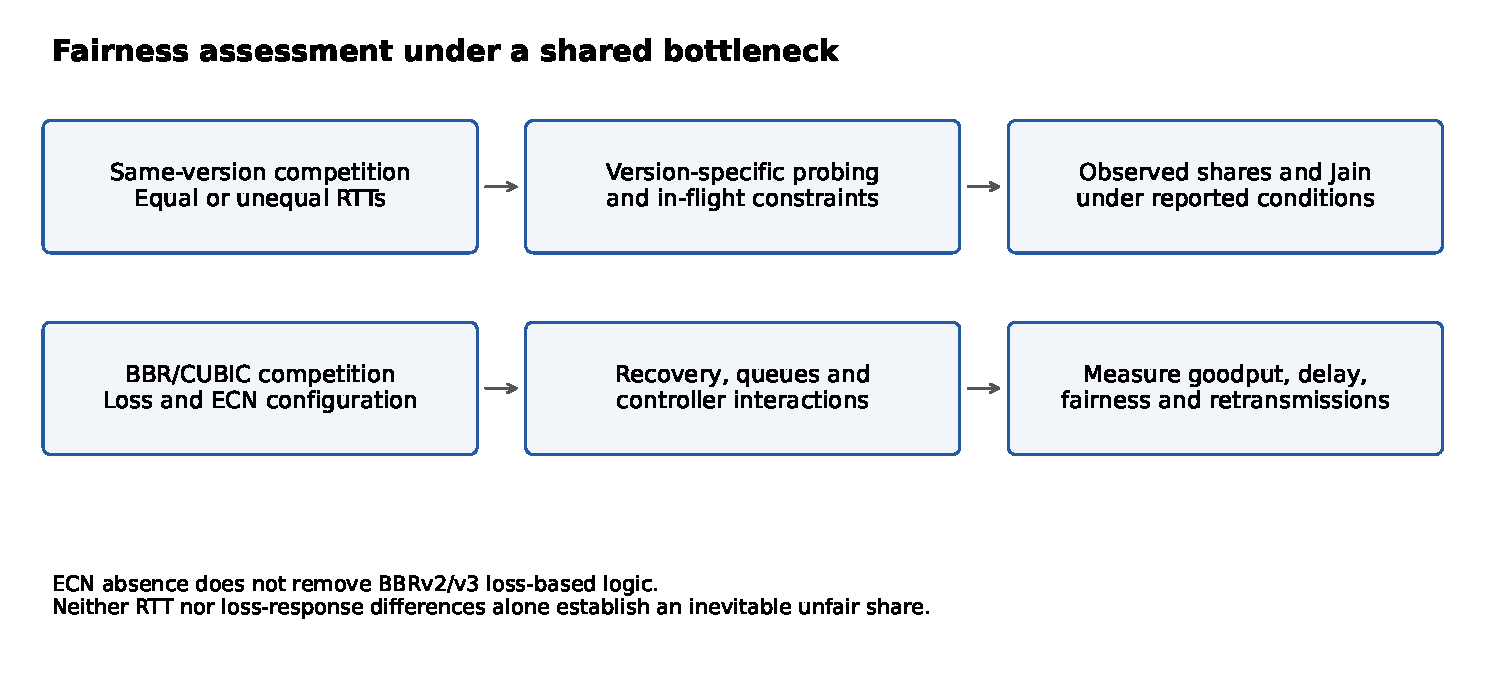
\includegraphics[width=\columnwidth]{fairness_mechanism_corrected.pdf}
  \caption{Assessment of same-version and BBR/CUBIC competition. Controller responses interact with queueing, recovery and the experiment configuration; fairness outcomes require measured per-flow rates. The original figure was generated with GPT Image 2.0 and manually checked by the authors; this replacement was drawn with Python/matplotlib using AI-assisted code preparation.}
  \label{fig:fairness_mech}
\end{figure}

\subsection{Formal Fairness Metrics}
\label{sec:fairness_metric}

Quantitative fairness assessment requires explicit metrics. The Jain Fairness
Index (JFI) proposed by \citet{jain1984fairness} is the primary tool for
measuring multi-flow bandwidth allocation in this paper:
\begin{equation}
  \label{eq:jfi}
  J(\mathbf{x}) = \frac{\left(\sum_{i=1}^{n} x_i\right)^2}{n \cdot \sum_{i=1}^{n} x_i^2}
\end{equation}
where $\mathbf{x}$ is the throughput vector of $n$ flows, $J=1$ indicates perfect
fairness, and $J=1/n$ indicates single-flow monopoly. In BBR analysis, JFI must
be combined with per-flow absolute throughput: when the number of flows is large,
the index may mask starvation of low-bandwidth flows~\citep{abrol2026bbr}.

\subsection{Intra-Protocol Fairness under Heterogeneous RTTs}
\label{sec:rtt_skew}

When multiple BBR flows compete at the same bottleneck, RTT heterogeneity can
produce unequal throughput shares, often disadvantaging short-RTT flows under
the conditions reported in prior measurements---a phenomenon commonly called
``RTT bias.'' \citet{hock2017bbr} first systematically reported this problem: at
$0.8\times$BDP buffer, short-RTT flows have a slight advantage; at $8\times$BDP,
long-RTT flow throughput can be several times that of short-RTT flows.
\citet{tao2018rtt} analyze RTT fairness using a queueing model. Any
predicted throughput ratio or fairness threshold depends on that model's
assumptions and must be checked against the experiment's queue, probing
and flow conditions. It is not interpreted here as a rule that an RTT
ratio above two inevitably produces a particular Jain index.

The per-flow BDP calculation relates two measured quantities:
\begin{equation}
  \label{eq:bdp}
  \mathrm{BDP}_i = \mathrm{BtlBw}_i \times \mathrm{RTprop}_i
\end{equation}
The longer-RTT flow has a larger $\mathrm{RTprop}_i$, so the in-flight amount
associated with a given measured delivery rate is larger. This relationship does
not by itself determine the flow's bandwidth share: probing duration, queue depth,
max-filter dynamics, version, queue management, and competing flow count also
matter. Within BBR's existing ``BtlBw$\times$RTprop'' measurement model,
adjusting gain parameters may change the observed bias under particular
conditions, but the equation alone is not a proof of inevitable long-RTT
dominance. A stronger mitigation may require changes to path-delay estimation or
additional network-side signals such as scalable ECN.

\begin{figure}[pos=htbp]
  \centering
  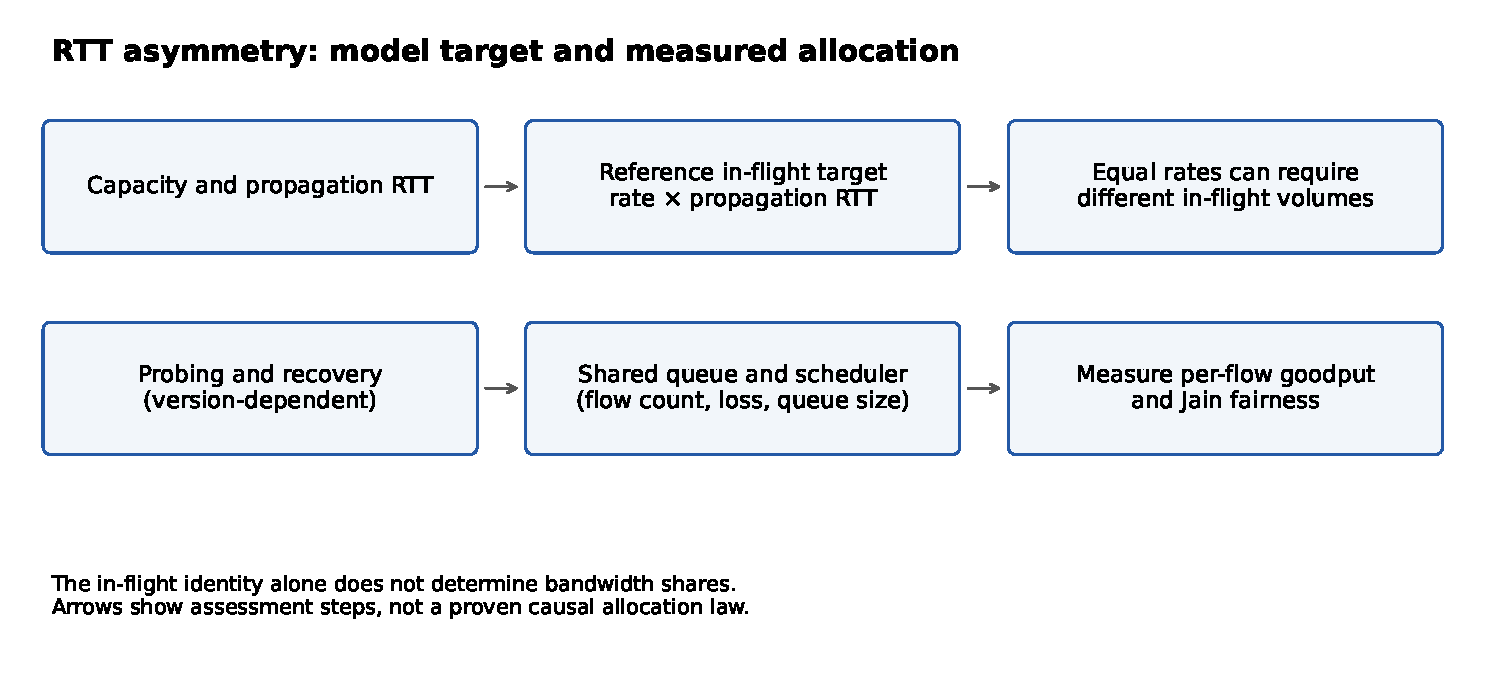
\includegraphics[width=\columnwidth]{rtt_skew_mechanism_corrected.pdf}
  \caption{RTT asymmetry separates the reference in-flight target from bandwidth allocation. Equal rates may require different in-flight volumes. Probing and shared-queue interactions must be evaluated through per-flow goodput and Jain fairness; no RTT-proportional share law is assumed. The original figure was generated with GPT Image 2.0 and manually checked by the authors; this replacement was drawn with Python/matplotlib using AI-assisted code preparation.}
  \label{fig:rtt_mechanism}
\end{figure}

BBRv2 attempts to mitigate intra-protocol unfairness by limiting inflight
when ECN marking or loss feedback exceeds a threshold~\citep{cardwell2019bbrv2}.
Without ECN marking, the ECN-derived component is unavailable, but loss-driven
updates and the associated state logic remain. BBRv3 further changes the
ProbeBW Down pacing behavior~\citep{cardwell2023bbrv3}. In Piotrowska's
multi-RTT evaluation, the BBRv3 Jain index varies across buffer settings and is
not uniformly higher than BBRv2; the exact values are conditional on that study's
topology and RTT distribution. The measured Jain values make version and queue configuration joint inputs
to the fairness assessment.

\begin{figure}[pos=htbp]
\centering
\captionsetup[subfigure]{skip=2pt}
\begin{subfigure}{0.48\columnwidth}
    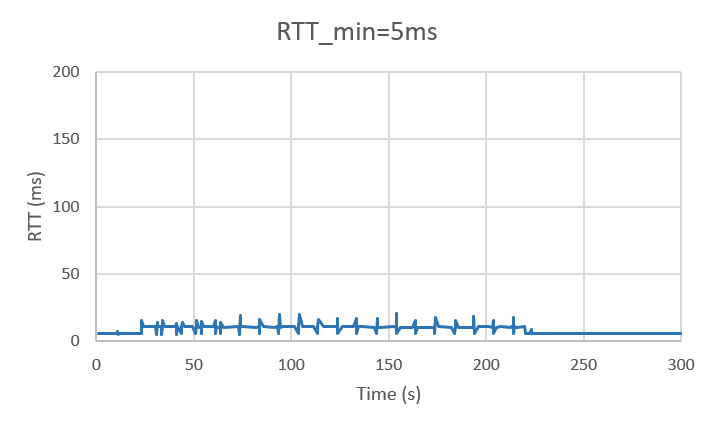
\includegraphics[width=\linewidth]{rtt_skew_rtt5ms.png}
    \caption{Longer-flow $\mathrm{RTT}_{\min}=5$\,ms ($\Delta$RTT\,=\,0\,ms, baseline)}
    \label{fig:rtt_a}
\end{subfigure}
\hfill
\begin{subfigure}{0.48\columnwidth}
    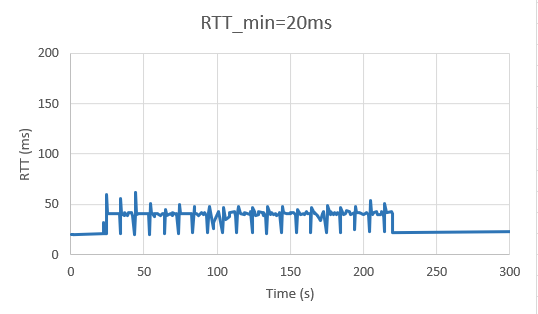
\includegraphics[width=\linewidth]{rtt_skew_rtt20ms.png}
    \caption{Longer-flow $\mathrm{RTT}_{\min}=20$\,ms ($\Delta$RTT\,=\,15\,ms)}
    \label{fig:rtt_b}
\end{subfigure}

\vspace{1em}

\begin{subfigure}{0.48\columnwidth}
    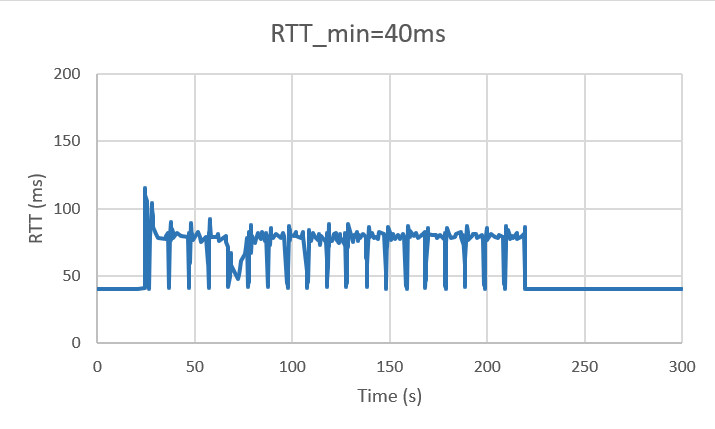
\includegraphics[width=\linewidth]{rtt_skew_rtt40ms.png}
    \caption{Longer-flow $\mathrm{RTT}_{\min}=40$\,ms ($\Delta$RTT\,=\,35\,ms)}
    \label{fig:rtt_c}
\end{subfigure}
\hfill
\begin{subfigure}{0.48\columnwidth}
    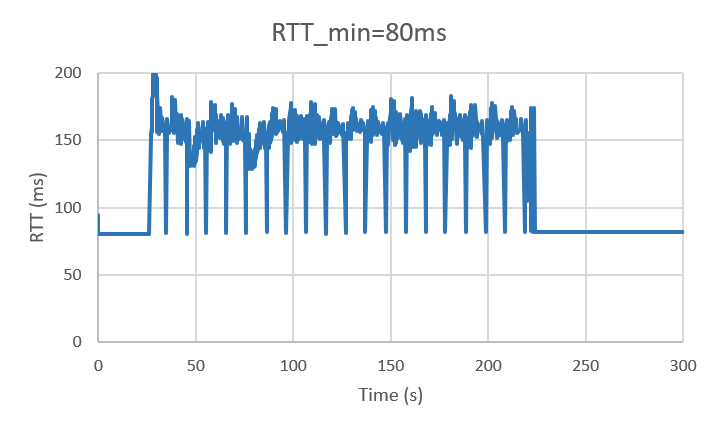
\includegraphics[width=\linewidth]{rtt_skew_rtt80ms.png}
    \caption{Longer-flow $\mathrm{RTT}_{\min}=80$\,ms ($\Delta$RTT\,=\,75\,ms)}
    \label{fig:rtt_d}
\end{subfigure}

\caption{RTT of the shorter-RTT flow under BBR two-flow competition. The vertical axes show RTT, including propagation and queueing components.
  The shorter flow has $\mathrm{RTT}_{\min}$ fixed at 5\,ms; the longer flow's
  $\mathrm{RTT}_{\min}$ varies from 5\,ms to 80\,ms, giving RTT differences of
  0, 15, 35, and 75\,ms respectively.
  Redrawn based on data from \citet{hock2017bbr}.}
\label{fig:rtt_skew}
\end{figure}

\subsection{Inter-Protocol Unfairness: Coexistence with CUBIC}
\label{sec:inter_fair}

When BBR and CUBIC coexist, buffer size, RTT configuration, and flow count
can affect their bandwidth shares. In the emulation study of
\citet{jaeger2019bbr}, Figure~10a varies the buffer with both flows at
50 ms RTT, Figure~10b varies their common RTT at a 2.3-BDP buffer,
and Figure~10c holds one flow at 50 ms while varying the other.
The reported fairness measure is the authors' throughput-based $F_{tp}$;
it should not be interchanged with Jain's index.

For that tested implementation, the authors report persistent BBR-induced
loss at buffer sizes up to about 1.5 BDP, approximately balanced shares
near the intermediate buffer range, and increasing CUBIC share as the
buffer grows further. These observations support a configuration-specific
buffer effect. They do not establish a universal 1.5- or 3-BDP threshold
for BBRv2, BBRv3, other queue policies, or arbitrary flow populations.
The cited survey literature provides context for these coexistence problems,
but a quantitative comparison requires the original study, implementation,
flow configuration, and metric definition to be identified.
\citet{zeynali2024bbrv3} further observed more extreme
results on real Internet paths: a single BBRv3 flow can occupy over 99\% of link
bandwidth (vs.\ 5 CUBIC flows) when ECN is enabled, and disabling ECN only
marginally reduces unfairness~\citep{zeynali2024bbrv3}.

\begin{figure}[pos=htbp]
  \centering
  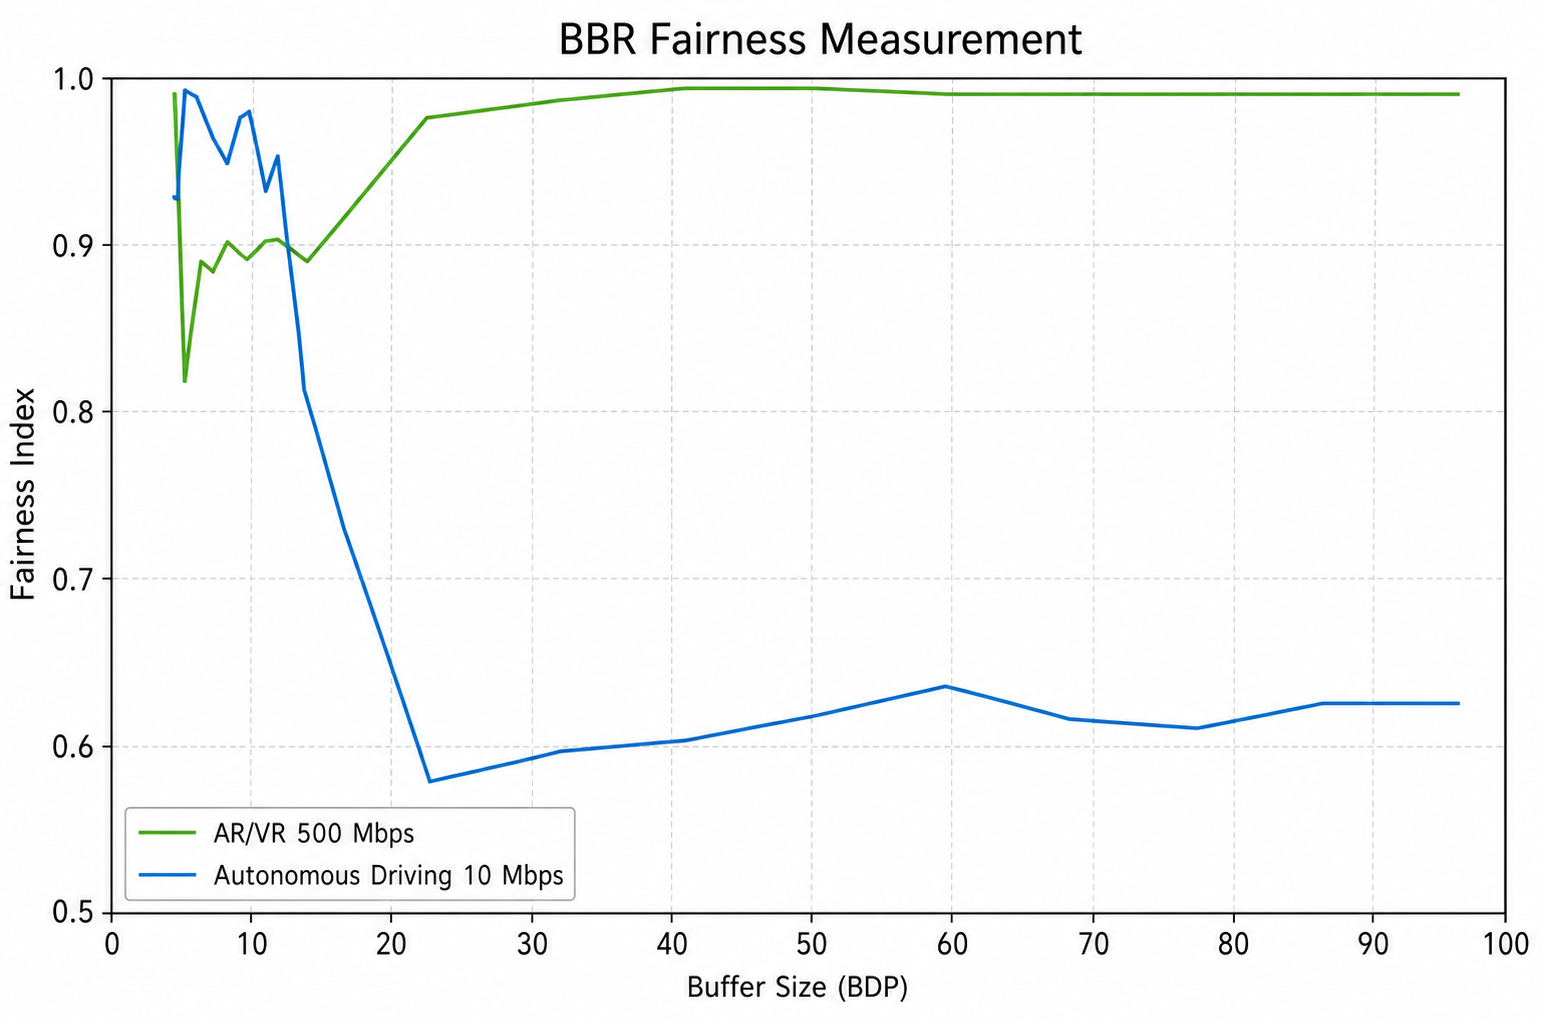
\includegraphics[width=0.8\columnwidth]{fairness_vs_buffer.png}
  \caption{Fairness variation of BBRv3 and CUBIC coexistence as a function of
    bottleneck buffer size \citep{abrol2026bbr}.}
  \label{fig:fairness}
\end{figure}

\subsection{Existing Remedies and Their Limits}
\label{sec:improvement}

For \textbf{intra-protocol fairness}, BBQ~\citep{ma2017fairness}\footnote{Published
as an arXiv preprint (arXiv:1706.09115); formal publication not confirmed at time
of review. Cross-validate with \citet{tao2018rtt}.} reduces probe cycles for
long-RTT flows; DA-BBR~\citep{kim2019delay} introduces a correction factor for
per-flow BDP; FaiRTT~\citep{abrol2024fairtt} achieves a Jain index of 0.98 in
ns-3 simulation, but robustness in real wireless networks is yet to be verified.
These approaches intervene through probing, operating-point estimation and
window control, offering distinct mechanisms for changing measured
allocation. Their comparisons should retain the tested implementation and
network conditions.

For \textbf{inter-protocol fairness}, Modest-BBR~\citep{zhang2018modest} scales
the congestion window after loss; BBR-CWS~\citep{song2020bbrcws} dynamically
adjusts the congestion window during loss recovery, but lacks response to
non-loss congestion signals (ECN). The IETF L4S standard~\citep{rfc9330}
represents another technical path: introducing a dual-queue structure and scalable
ECN congestion signals at the network side to support both low latency and high
throughput---complementary to, rather than a replacement for, end-side algorithm
iteration.

Table~\ref{tab:fairness_versions} connects version-specific mechanisms
to reported sharing behavior.
Estimator design, probing dynamics, loss responses and queue management
should be evaluated jointly with per-flow rates and explicit measurement
conditions.

\begin{table}[pos=htbp]
  \caption{Summary of fairness improvement trajectory across BBRv1/v2/v3.}
  \label{tab:fairness_versions}
  \small
  \begin{tabularx}{\tblwidth}{@{}p{1.0cm}p{2.3cm}p{2.3cm}p{2.0cm}X@{}}
    \toprule
    \textbf{Version} & \textbf{Intra-protocol} & \textbf{Inter-protocol}
      & \textbf{Key improvement} & \textbf{Assessment considerations} \\
    \midrule
    BBRv1 & RTT-dependent shares under reported queue/probing conditions &
      BBR/CUBIC shares vary with buffer, RTT and flow count & --- &
      Cwnd-derived inflight limit remains; loss response differs from v2/v3 \\
    \midrule
    BBRv2 & Conditional improvement under the reported configurations &
      Improved under some ECN-enabled configurations &
      ECN triggers $\mathrm{inflight\_hi}$ constraint &
      ECN-derived feedback is unavailable on non-ECN paths; loss-driven logic remains \\
    \midrule
    BBRv3 & \textbf{Fairness remains configuration-dependent with deep queues} &
      No universal improvement over v2 established &
      Version-specific probing and loss-response changes &
      Reported fairness limitations require their tested implementation and queue conditions \\
    \bottomrule
  \end{tabularx}
\end{table}

\FloatBarrier

% ============================================================
\section{Engineering Obstacles and AI-Enhanced Directions}
\label{sec:deployment}
% ============================================================

\subsection{Engineering Deployment and Structural Obstacles}
\label{sec:engineering}

Deployment comparisons evaluate parameter tuning, estimator changes and
network-side mechanisms under the same stated performance requirements.
The relevant outcomes are per-flow rates, delay, retransmissions and
operating cost.

BBR has moved from experimental scheme to large-scale engineering deployment since
2016: Google B4 and YouTube/CDN public observations show it can improve
utilization, reduce latency, and alleviate
Bufferbloat~\citep{cardwell2017bbr}; the Linux kernel and IETF drafts drive v1--v3
continuous evolution~\citep{cardwell2017bbr,cardwell2019bbrv2,ietf_ccwg_bbr,abrol2026bbr};
and Starlink-class link measurements show BBR has potential advantages on LEO
satellite paths, but with strong dependence on terminal, tunnel, and switching
conditions~\citep{deutschmann2023starlink,kamel2024starquic}.

Deployment assessment should examine feedback availability, wireless
measurement conditions and application requirements separately.

A deployment consideration is the availability of explicit congestion
feedback. ECN marking requires support at the endpoints and along the path,
and L4S additionally depends on its queueing and endpoint requirements
\citep{rfc3168,rfc9330,rfc9331,rfc9332}. Without marking, the ECN-derived
component is unavailable, but BBRv2/v3 retain loss-driven updates and
version-specific state logic. Performance under that configuration must be
measured; absence of ECN does not establish reversion to BBRv1 or a fixed
loss of fairness.

The second obstacle is \textbf{multiple incompatibilities in wireless environments},
each with a different root cause, making a single fix insufficient. An underestimated RTprop
can reduce the model-derived in-flight target and delivered throughput~\citep{abrol2026bbr}; pacing and local queue constraints can limit WiFi frame
aggregation in the tested 802.11n/ac settings (see \S\ref{sec:wireless_loss}); and the time-scale mismatch between
wireless/LEO link variation and BBR's multi-RTT probing windows can cause
measurement model estimates to lag channel state changes~\citep{wang2024bbr_leo,kamel2024starquic,laniewski2024road}.

The third obstacle is the \textbf{absence of heterogeneous flow QoS guarantees}.
Bandwidth fairness alone does not establish latency or reliability guarantees
for heterogeneous applications. Claims about URLLC suitability require
application-level deadlines, loss budgets and scheduling conditions;
a bulk two-flow result does not supply those guarantees.

\subsection{Classification Evaluation of AI-Enhanced Approaches}
\label{sec:ai}

Evidence on learning-assisted control should distinguish the action space
and evaluation environment. \citet{xiao2019tcpdrinc} learn congestion-window
actions in ns-3 using a goodput--delay utility difference. In their dynamic
simulation, Table~2 reports a mean Jain index of 0.8058 and a 95\%
confidence interval of [0.7233, 0.8882]. The baseline intervals overlap,
and the table alone does not establish statistically superior fairness.
The authors also report that performance is best near the training
parameters. These observations motivate explicit tests of transfer and inference
cost. The comparison concerns the reported baseline set, which excludes BBR.


Learning-based methods should be assessed by their observations, actions,
objectives and evaluation settings. Learning a local BBR parameter differs
from replacing the controller policy or coordinating several flows.

\begin{table}[pos=tbp]
  \caption{Comparison of representative AI-assisted congestion control approaches
    ($\bigstar$: BBR-specific works).
    Remy~\citep{winstein2013remy}; PCC~Vivace~\citep{dong2018vivace};
    Aurora~\citep{jay2019aurora}; OI-BBR~\citep{kim2020ml};
    Symbolic-PCC~\citep{sharan2022symbolic}; MARLIN~\citep{galliera2023marlin};
    Mutant~\citep{pappone2025mutant}; RL-BBR~\citep{ketabi2023drl}.}
  \label{tab:aicc}
  \footnotesize
  \setlength{\tabcolsep}{2pt}
  \begin{tabularx}{\tblwidth}{@{}p{2.1cm}p{1.8cm}p{0.9cm}p{1.1cm}p{0.7cm}XX@{}}
    \toprule
    \textbf{Method} & \makecell[l]{\textbf{AI paradigm}} & \makecell[l]{\textbf{Ctrl}\\\textbf{level}}
      & \makecell[l]{\textbf{Testbed}} & \makecell[l]{\textbf{In-}\\\textbf{terp.}}
      & \textbf{Key contribution} & \textbf{Evaluation scope and deployment requirements} \\
    \midrule
    Remy & Offline opt. & Policy & Sim & Low & Auto-generated CC policy & Requires prior distribution \\
    PCC Vivace & Online learning & Policy & R+S & Low & Utility-driven control & Slow convergence \\
    Aurora & DRL & Policy & Sim & Low & Multi-scenario generalization & Sim2Real gap \\
    $\bigstar$ OI-BBR & Decision tree & Assist & Mininet & \textbf{High} & Interpretable rule learning & Discrete decisions only \\
    Symbolic-PCC & DRL+sym.\ distill. & Param & Sim+tb & Med & Symbolic rules from NN & Limited expressiveness \\
    MARLIN & Max-ent.\ RL & Policy & R+S & Low & Mitigates Sim2Real gap & High complexity \\
    $\bigstar$ Mutant & Online RL+imit. & Policy & Real & Low & No offline training & Stability concerns \\
    $\bigstar$ RL-BBR & DRL & Param & DC & Low & DC throughput optimization & Narrow scope \\
    \bottomrule
  \end{tabularx}
\end{table}

One research direction is learning-assisted local estimation and
decision-making: \citet{ketabi2023drl} use DRL to adjust
pacing\_gain and cwnd\_gain; OI-BBR~\citep{kim2020ml} uses a decision tree to
learn ``when to yield to CUBIC.'' Local parameter changes preserve more of the underlying controller than
a full policy replacement. Potential uses include RTprop estimation
calibration, WiFi frame-aggregation identification and ProbeRTT timing; their applicability depends on the available signals, action space and
evaluation conditions. Local parameter learning is evaluated against fixed heuristics and broader
policy changes using per-flow rates, delay and operating cost.

Policy-level learning schemes explore a wider action space than local
parameter adjustment~\citep{winstein2013remy,dong2018vivace,jay2019aurora,galliera2023marlin,pappone2025mutant}.
Their deployment assessment should report inference time, training cost,
controller stability and performance outside the training distribution.
Network-level methods such as GraphCC and LLM-CC require a separate
assessment of coordination scope and decision frequency
\citep{bernardez2025graphcc,huang2024llm}. Deployment evaluation pairs control performance with measured inference
latency at the intended decision frequency.

\subsection{Core Open Challenges}
\label{sec:ai_challenges}

The reviewed evaluations leave several questions for deployment. First,
throughput--delay utility is not equivalent to an explicit fairness or
service-priority objective. TCP-Drinc reports Jain fairness, but its
baseline intervals overlap and its evaluation does not include BBR.
A study's reported metrics must therefore be distinguished from the
objectives used to train its policy; we make no claim that all learning
methods optimize only one objective or that none can address fairness.

Second, interpretability should be evaluated alongside performance and
operational safeguards. A decision tree exposes rules more directly than
a neural policy, but neither representation alone proves stability or
justifies deployment. Third, an evaluation in ns-3 or Mininet is limited
by the topology, traffic, channel and timing models actually configured,
not by an inherent inability of those tools to model dynamic paths.
Transfer claims need tests outside the training conditions, including
heterogeneous traffic and path changes~\citep{jiang2021mlcc}.
Finally, wireless and LEO evaluations should test changes in capacity,
delay and loss, as well as adaptation time and retained performance
\citep{kamel2024starquic,laniewski2024road}. These are evaluation questions,
not a proof of a universal ceiling on learning-assisted control.

\subsection{Technical Roadmap}
\label{sec:ai_roadmap}

The reviewed evidence motivates two complementary research directions,
without excluding other designs. The near-term path is a ``model-driven + limited data-driven'' hybrid
framework: keep the BBR state machine auditable, and limit learning modules to
local sub-problems such as RTprop calibration, WiFi frame aggregation detection,
or ProbeRTT timing adjustment. A complementary direction is network-side congestion feedback. L4S dual
queues and scalable ECN (RFC~9330~\citep{rfc9330}) require compatible
endpoint behavior. Whether a BBR implementation meets those requirements
and improves fairness must be evaluated; L4S support alone does not
establish that outcome. The former improves end-side measurement
accuracy, the latter improves network-side signal quality; they are complementary,
not alternatives.

% ============================================================
\section{Controlled Experiments}
\label{sec:controlled_experiments}

\subsection{Implementation identity and experimental design}
We use E1 to examine bandwidth sharing between two flows of the same
implementation as RTT asymmetry and queue depth change, and E2 to examine
coexistence with CUBIC. E3 extends the equal-RTT comparison across capacity
and propagation delay. An artificial-loss extension separates configured
access-link loss from bottleneck congestion. These tests evaluate the
framework's assessment dimensions under stated conditions, Each experiment addresses a separate assessment question.

The Linux emulation uses Mininet 2.3.0, Open vSwitch bridges, iperf3 3.9
and iproute2 5.15.0. Two sender hosts connect through switches $s_1$ and
$s_2$ to one receiver: $h_1,h_2\rightarrow s_1\rightarrow s_2\rightarrow h_3$.
The $s_1$--$s_2$ link is the bottleneck, configured with a token-bucket
rate limiter and child netem FIFO packet limit, without AQM or ECN.
The receiver access link supplies the base propagation delay; additional
delay on the second sender's access link creates RTT asymmetry. Each
sender opens one TCP connection to a separate receiver port (5201 or
5202), with one-second iperf3 reporting intervals. The topology is rebuilt
between runs. The MTU is 1,500 bytes. In E1/E2, the reference BDP is
$100\,\mathrm{Mbps}\times20\,\mathrm{ms}/8=250,000$ bytes, using the first
flow's configured propagation RTT, including when the second RTT differs.
Queue targets of 125,000, 500,000 and 2,500,000 bytes are rounded up to
84, 334 and 1,667 MTU-sized packets, respectively.

The archived experiments comprise 340 two-flow runs: 60 each for the
Ubuntu 5.15.0-181-generic in-tree baseline, the separately loaded BBRv1 module, BBR2, and
BBRv3; 80 E3 runs; and 20 artificial-loss runs. The manifests identify
BBRv3 by the 6.13.7-bbr3 kernel, source marker BBR\_VERSION=3, and runtime
name \texttt{bbr}. The BBRv1 module registers as \texttt{bbr1} and uses
a recorded compatibility patch for an unexported TSO helper. BBR2 uses
a separate 5.13.12-bbr2alpha kernel and runtime name \texttt{bbr2}.
The in-tree baseline remains a distinct implementation label.
Different kernel environments and the module patch limit causal
attribution of performance differences to algorithm version alone.

The E1/E2 matrix uses a 100-Mbps bottleneck, a 20-ms first-flow RTT,
second-flow RTTs of 20, 40, or 80 ms for the same-algorithm comparison,
and equal-RTT BBR/CUBIC competition. Queue targets are 0.5, 2, or 10
times the reference BDP. Each condition has five 180-s repetitions,
with ECN disabled. Receiver-side iperf3 summaries provide the archived
full-run goodput. Jain fairness and flow shares are derived from those
per-flow rates. For each run, with receiver rates $x_1,x_2$, we compute
$G=x_1+x_2$, $J=(x_1+x_2)^2/[2(x_1^2+x_2^2)]$ and
$S_2=x_2/(x_1+x_2)$. Reported Jain indices and shares are means of
these run-level quantities, rather than values calculated from mean rates.
In E2, flow 1 is BBR and flow 2 is CUBIC, so the mean BBR share is
$1-\overline{S_2}$. Receiver goodput excludes protocol headers; therefore
it need not equal the configured link rate. The supplement supplies
per-run values and variability; five repetitions support descriptive
comparisons, not population-wide significance claims.

The configuration declares a 30-s warmup; the primary archived analysis
uses the complete receiver summary. A separate sensitivity analysis uses
complete receiver intervals within the configured 30--180-s window,
without estimating bytes in boundary intervals. Across 68 condition
summaries, the largest absolute changes in mean total goodput, Jain
index, and second-flow share are 1.313 Mbps, 0.02949, and 0.01678,
respectively. The separate window analysis quantifies the sensitivity of these summaries.

Loaded RTT measurements are sequential early ping samples from the two
senders. Queue counters were sampled before the transfers completed.
The RTT and queue observations use different windows from the receiver
goodput summary; their values are reported as complementary measurements.

\subsection{Conditioned cross-version comparison}
Across the tested 100-Mbps matrix, equal-RTT total goodput remains close to
the bottleneck for all four implementations, while flow shares and Jain
fairness vary with RTT asymmetry, queue setting, and implementation. Under
the 40- and 80-ms second-flow conditions, the observed long-RTT share differs across implementations. E1 quantifies allocation under RTT asymmetry; E2 evaluates coexistence
with CUBIC at equal RTTs in the documented implementation environments.

For the no-ECN BBR/CUBIC comparison, total goodput is similar across the
four implementation environments, while the BBR/CUBIC share and Jain
index remain condition dependent. The experimental supplement contains the per-run rates, condition
summaries and plotting scripts.

\begin{figure}[htbp]
\centering
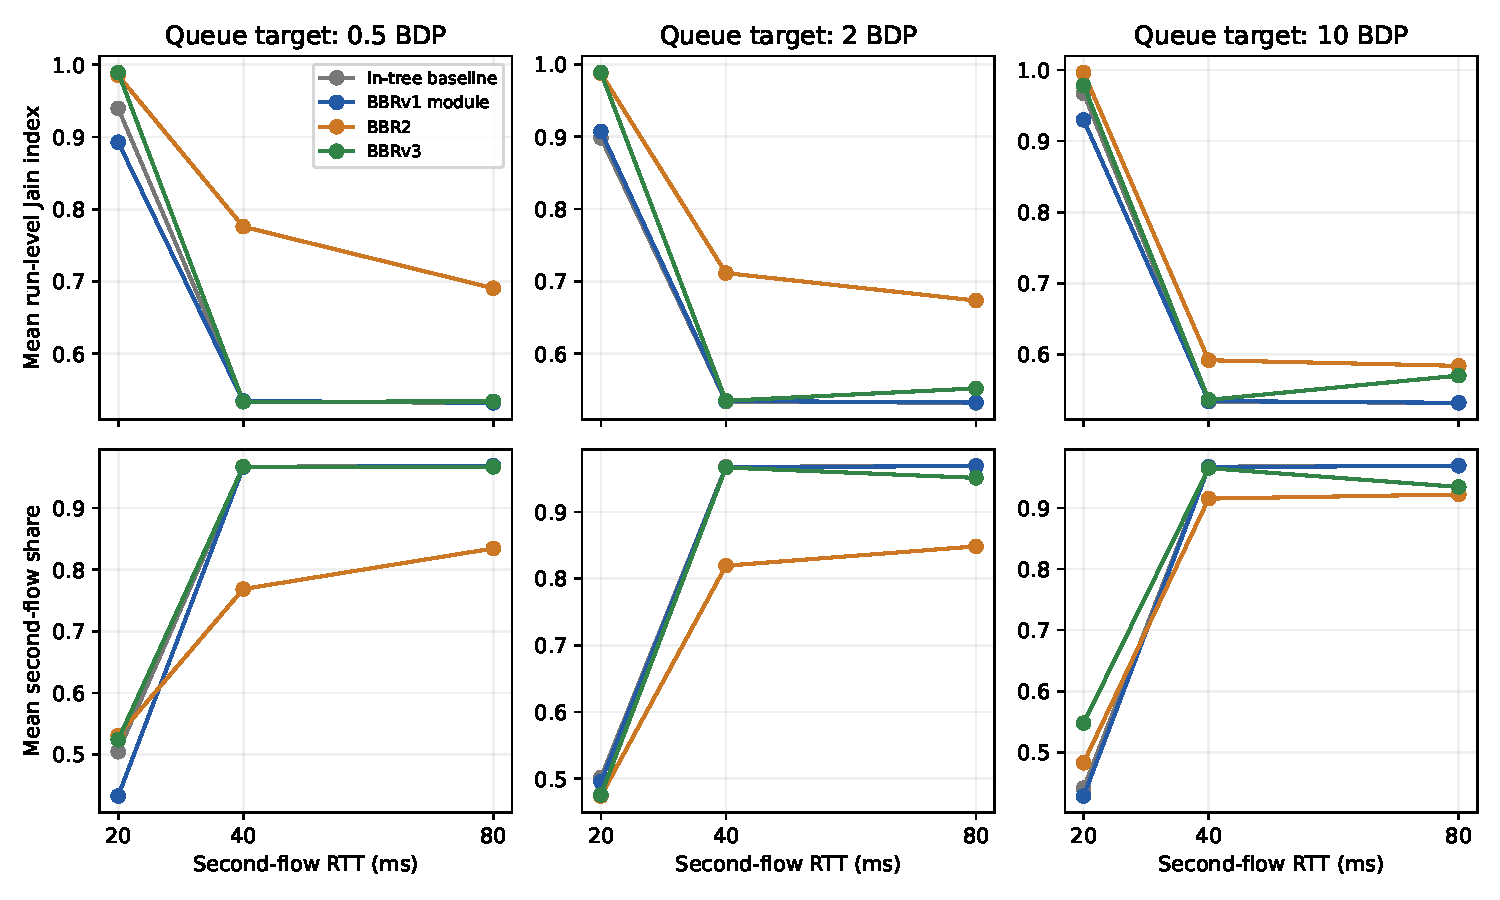
\includegraphics[width=\linewidth]{e1_results.pdf}
\caption{E1 two-flow comparison at 100 Mbps, with first-flow RTT 20 ms and ECN disabled. Curves show means of five run-level Jain indices and second-flow shares, not indices computed from averaged rates. Queue targets use the reference BDP.}
\label{fig:e1_results}
\end{figure}

\begin{table}[htbp]
\centering
\caption{E2 competition with CUBIC at 100 Mbps and equal 20-ms RTTs, with ECN disabled. Each cell summarizes five full-run receiver measurements. Share denotes the BBR flow; Jain is the mean of per-run indices. Different implementation environments limit causal version attribution.}
\label{tab:e2_results}
\small
\begin{tabular}{lrrrr}
\toprule
Implementation & Q/BDP & Total (Mbps) & BBR share & Jain \\
\midrule
In-tree baseline & 0.5 & 95.59 & 0.155 & 0.677 \\
In-tree baseline & 2 & 95.59 & 0.153 & 0.674 \\
In-tree baseline & 10 & 95.58 & 0.165 & 0.690 \\
BBRv1 module & 0.5 & 95.59 & 0.144 & 0.663 \\
BBRv1 module & 2 & 95.59 & 0.143 & 0.663 \\
BBRv1 module & 10 & 95.59 & 0.149 & 0.669 \\
BBR2 & 0.5 & 95.58 & 0.278 & 0.835 \\
BBR2 & 2 & 95.58 & 0.327 & 0.886 \\
BBR2 & 10 & 95.58 & 0.274 & 0.828 \\
BBRv3 & 0.5 & 95.58 & 0.153 & 0.675 \\
BBRv3 & 2 & 95.58 & 0.145 & 0.664 \\
BBRv3 & 10 & 95.59 & 0.164 & 0.689 \\
\bottomrule
\end{tabular}
\end{table}


Table~\ref{tab:e2_results} shows that similar total goodput does not imply
similar bandwidth allocation. Total rates are 95.58--95.59 Mbps in this
matrix, while the BBR share is 0.143--0.327. BBR2 obtains shares of
0.274--0.327 and Jain indices of 0.828--0.886; the BBRv1 module and
BBRv3 obtain smaller shares in these particular runs. The implementation environments and no-ECN configuration identify the
scope of these comparisons.

For unequal-RTT E1 cases, the second flow receives substantially more than
half the goodput in the tested matrix (Figure~\ref{fig:e1_results}). The
size of the imbalance varies with implementation and queue setting: across
the 24 unequal-RTT conditions, the mean long-RTT share ranges from
0.769 to 0.969, and mean Jain fairness from 0.532 to 0.776.
These measured shares make allocation an explicit assessment outcome,
alongside the aggregate rate and the reported path conditions.

\subsection{Additional comparison under equal RTT}
The additional experiment matrix contains eight network cases at 50 or
200~Mbps, 10 or 60~ms RTT, and two frozen buffer labels.
For the 50-Mbps cases, the configured absolute buffers correspond
to 4 and 16 times the physical reference BDP, although the frozen file
labels them 1 and 4. For the 200-Mbps cases, those labels are consistent
with the capacity-times-reference-RTT BDP. The original predictions
are retained; the affected cases do not validate the intended buffer bins. We ran two BBRv3 flows
and two CUBIC flows separately for five independent repetitions per case
(80 runs in total). ECN is disabled in all cases.

Table~\ref{tab:e3_candidate} reports mean total goodput and Jain fairness.
E3 extends the rate/fairness assessment across two capacities and two
RTTs. Mean BBRv3 Jain indices range from 0.995 to 1.000, compared with
0.917 to 0.987 for CUBIC; the table reports the corresponding goodput
values together, making both utilization and sharing visible. The queue snapshots do not cover the complete measurement window;
The receiver summary, sender retransmissions and queue snapshot provide
separate indicators for the documented operating conditions.
The archived goodput and Jain values use full-run receiver summaries.
A separate post-warmup interval sensitivity analysis is retained;
the table reports the complete receiver summary; window sensitivity is
provided separately.

\begin{table}[htbp]
\centering
\caption{Descriptive E3 full-run means. Goodput (Mbps) and Jain cells report BBRv3/CUBIC. C is Mbps and RTT is ms. Buffer uses decimal kB; actual target Q/BDP is computed from capacity and reference RTT, before packet-limit rounding. Frozen labels are preserved in the input audit.}
\label{tab:e3_candidate}
\begin{tabular}{lrrrrrr}
\toprule
Case & C & RTT & Buffer (kB) & Actual Q/BDP & Goodput & Jain \\
\midrule
E3\_001 & 50 & 10 & 250 & 4 & 47.1/47.8 & 1.000/0.969 \\
E3\_002 & 50 & 10 & 1000 & 16 & 47.2/47.8 & 1.000/0.917 \\
E3\_003 & 50 & 60 & 1500 & 4 & 46.9/47.7 & 1.000/0.928 \\
E3\_004 & 50 & 60 & 6000 & 16 & 46.8/47.7 & 1.000/0.987 \\
E3\_005 & 200 & 10 & 250 & 1 & 188.2/191.2 & 0.995/0.963 \\
E3\_006 & 200 & 10 & 1000 & 4 & 188.0/191.2 & 0.999/0.955 \\
E3\_007 & 200 & 60 & 1500 & 1 & 187.0/190.8 & 0.997/0.963 \\
E3\_008 & 200 & 60 & 6000 & 4 & 187.1/190.8 & 0.996/0.938 \\
\bottomrule
\end{tabular}
\end{table}


\subsection{Goodput under artificial access-link loss}
The artificial-loss extension compares BBRv3 and CUBIC at configured
loss probabilities of zero and 0.1\% on a separate access link. Each run
uses two flows of the same algorithm, a 100-Mbps bottleneck, equal 20-ms
RTTs and a 500,000-byte queue target (2 reference BDP),
with five runs per algorithm and loss setting. Archived full-run mean total
goodput changes from 93.87 to 94.25 Mbps for BBRv3 and from 95.58 to
81.06 Mbps for CUBIC. The small BBRv3 increase is a descriptive observation
and is not evidence that loss improves performance. The loss generator's
seed was not exposed in the retained configuration; this setup does not
represent correlated wireless or satellite errors.

The additional equal-RTT cases extend the capacity and RTT settings of
the main matrix. Their physical queue sizes are reported explicitly in
Table~\ref{tab:e3_candidate}. Because four cases differ from the intended
buffer labels, we use these results as an additional empirical comparison,
rather than as a validation of the original buffer-category predictions.
The experiments evaluate goodput and bandwidth sharing under controlled
conditions; they do not establish universal suitability thresholds or
isolate the causal effect of an individual controller mechanism.

\subsection{Quantitative Transfer Evaluation of the Framework}
\label{sec:framework_transfer}

We supplement the scenario comparisons with a quantitative test of whether
an equal-RTT calibration transfers to different capacities and delays.
This analysis was designed during revision after the archived results were
available. Calibration and evaluation runs are disjoint, but the test is
retrospective; its design and data split are documented in the supplement.
The analysis script retains all inputs and reports the constant-baseline
comparison, including the contribution of queue conditioning.

Calibration uses only the 15 BBRv3 E1 runs with equal 20-ms RTTs at
100 Mbps, five at each queue target $q\in\{0.5,2,10\}$. At each target,
we estimate mean $u$ and mean $J$. For a target queue ratio between knots,
we linearly interpolate the two means in $\log q$; outside the range,
we extend the adjacent segment and restrict predictions to the metric's
feasible interval. The comparator predicts the overall calibration mean,
independent of queue size. Neither model fits an E3 outcome. Capacity and
RTT effects cannot be estimated from this single-capacity, equal-RTT
calibration; transferring normalized rates therefore tests an explicit
assumption that the evaluation tests.

The primary transfer comparison uses the four 200-Mbps E3 cases, where
physical queue ratios agree with the frozen input labels: RTTs of 10 or
60 ms and $q\in\{1,4\}$. The four 50-Mbps cases are a separate comparison
using their corrected physical ratios of 4 and 16. Errors are computed
against each condition's five-run mean, for 20 BBRv3 runs in each group.
The 40 CUBIC runs remain a performance comparator and are not calibration
data for the BBRv3 predictor.

\begin{table}[htbp]
\centering
\small
\caption{Retrospective transfer errors for BBRv3 condition means. MAE is the
mean absolute error; normalized-goodput errors are fractions of capacity.
Queue interpolation uses E1 only. The constant predictor uses the same
calibration data. Each row evaluates four E3 conditions.}
\label{tab:framework_transfer}
\begin{tabular}{llrrr}
\toprule
Evaluation group & Metric & Queue MAE & Constant MAE & Queue max. error \\
\midrule
200 Mbps, actual $q=1,4$ & $u$ & 0.00264 & 0.00264 & 0.00400 \\
 & $J$ & 0.01010 & 0.01134 & 0.01464 \\
50 Mbps, actual $q=4,16$ & $u$ & 0.00309 & 0.00309 & 0.00366 \\
 & $J$ & 0.02027 & 0.01444 & 0.02499 \\
\bottomrule
\end{tabular}
\end{table}

Table~\ref{tab:framework_transfer} separates modest transfer error from
predictive added value. In the four input-matched cases, the queue-conditioned
Jain estimate has slightly smaller MAE than the constant predictor, but
normalized-goodput MAE is the same to the displayed precision. In the corrected 50-Mbps cases, Jain MAE is 0.02027 for queue
interpolation and 0.01444 for the constant estimate. This comparison
identifies the dependence of transfer estimates on their conditioning
variables. The largest Jain error is about
0.025; reporting only high aggregate utilization would conceal this
assessment limitation. These results quantify the framework's transfer
boundary without claiming that E3 validates the original queue thresholds.

We also instantiate the analytical assessment in
Section~\ref{sec:analytical_assessment} with illustrative requirements
$u_0=0.90$ and $j_0=0.95$. These values were selected for retrospective
illustration, not frozen as experimental acceptance thresholds. All 40
BBRv3 and all 40 CUBIC E3 runs meet the utilization requirement, while
40 BBRv3 and 27 CUBIC runs meet both requirements. The result is restricted
to equal-RTT same-algorithm competition; E2 provides the separate coexistence
assessment. The supplement reports
run-level decisions and a threshold sensitivity grid. Receiver-goodput and early-ping windows are reported separately. Sender
retransmission totals and queue snapshots provide complementary indicators
for the documented operating conditions.

\begin{table}[htbp]
\centering
\small
\caption{Sensitivity of the retrospective E3 rate/fairness assessment to
illustrative service requirements. Cells count runs meeting both limits,
from 40 runs per algorithm. They are not independent condition counts.}
\label{tab:assessment_requirements}
\begin{tabular}{rrrr}
\toprule
Minimum $u$ & Minimum $J$ & BBRv3 & CUBIC \\
\midrule
0.90 & 0.95 & 40/40 & 27/40 \\
0.95 & 0.95 & 0/40 & 27/40 \\
0.90 & 0.99 & 38/40 & 19/40 \\
\bottomrule
\end{tabular}
\end{table}

The higher utilization requirement in Table~\ref{tab:assessment_requirements}
reverses which algorithm meets the joint requirement more often: no
BBRv3 run reaches $u=0.95$, whereas all CUBIC runs do. Tightening fairness
instead reduces both algorithms' pass counts. This measured throughput--allocation tradeoff makes the service
preference explicit under equal RTTs. The full
threshold grid and per-condition variability are provided in the supplement.

The frozen F07 predictions are retained separately from this new analysis.
They specify qualitative ``near-capacity'' or ``near-one'' outcomes without
numerical acceptance margins, and request medians rather than the reported
full-run means. Four cases also have inconsistent physical queue inputs.
The new transfer test reports numerical error directly; the historical
prediction sheet remains in the supplement as a separate record.


\FloatBarrier

\section{Conclusion}
\label{sec:conclusion}
% ============================================================

This survey connects BBR version evolution, network conditions and
performance objectives through a common assessment. Buffer depth, BDP and
loss source organize the evidence; capacity, RTT, implementation, queue
management and competing flows make each comparison interpretable. The
analytical procedure translates fairness requirements into flow-share
constraints and assesses utilization, delay, fairness and retransmission
cost separately.

The 340-run evaluation makes the distinction between utilization and
allocation concrete. In twelve BBR/CUBIC conditions, total goodput stays
within 95.58--95.59 Mbps while the BBR share ranges from 0.143 to 0.327.
Under unequal RTTs, measured long-RTT shares range from 0.769 to 0.969.
The additional equal-RTT cases expose a throughput--fairness tradeoff:
changing the stated service requirements changes which runs meet the
joint assessment. These results place per-flow outcomes alongside the
aggregate rate that otherwise conceals them.

For deployment assessment, the central lesson is to report the path and
implementation conditions, measure each required outcome, and make service
requirements explicit. The retained measurements and analysis support
that assessment under the documented conditions. Learning-assisted control
can be evaluated within the same structure by connecting its objectives
and actions to measured allocation, delay and operating cost. A useful
BBR comparison therefore explains both how much traffic the link carries
and how that capacity is shared.

% ============================================================
\section*{Acknowledgements}
This research did not receive any specific grant from funding agencies in the
public, commercial, or not-for-profit sectors.
% Replace with actual funding information if applicable.

\section*{Declaration of competing interest}
The authors declare that they have no known competing financial interests or
personal relationships that could have appeared to influence the work reported
in this paper.

\section*{Data availability}
The revision includes new controlled-network measurements alongside published
studies. Raw per-run configurations and logs, implementation manifests,
analysis scripts and condition summaries are provided in the accompanying
experimental supplement. Search exports and screening records are provided
in a separate search supplement. No public archive DOI is claimed.

\section*{Declaration of generative AI and AI-assisted technologies in the
manuscript preparation process}
% Original draft named ChatGPT/GPT-5.5 and several uses, but those facts
% have not been confirmed by the authors or original figure creators.
During preparation of the original manuscript, the authors used OpenAI
GPT Image 2.0 to generate Figures 3--6 and manually checked their technical
content. During this revision, AI assistance was used for manuscript editing
and preparation of plotting code. Figures 2--6 were redrawn using retained
Python plotting scripts to correct delay labels, distinguish controller
versions, and remove unsupported bandwidth-allocation inferences.
The authors take responsibility for the manuscript content.

\printcredits

\bibliographystyle{elsarticle-num-names}
\bibliography{refs}

\end{document}
